\documentclass[12pt, a4paper]{article}

% --- Packages ---
\usepackage[utf8]{inputenc}
\usepackage[T1]{fontenc}
\usepackage{geometry}
\geometry{a4paper, margin=1in, headheight=15pt}
\usepackage{xcolor}
\usepackage{hyperref}
\usepackage{graphicx}
\usepackage{tcolorbox}
\usepackage{fancyhdr}
\usepackage{titlesec}
\usepackage{enumitem}
\usepackage{parskip}
\usepackage{caption}
\usepackage{float}
\usepackage{listings}

% --- Colors ---
\definecolor{primary}{RGB}{12, 74, 110}     % Dark Slate Blue
\definecolor{secondary}{RGB}{2, 132, 199}   % Sky Blue
\definecolor{accent}{RGB}{240, 249, 255}    % Very Light Blue for backgrounds
\definecolor{darkgray}{RGB}{71, 85, 105}
\definecolor{codebg}{RGB}{248, 250, 252}

% --- Hyperref Setup ---
\hypersetup{
    colorlinks=true,
    linkcolor=primary,
    filecolor=secondary,      
    urlcolor=secondary,
    pdftitle={Comprehensive Week 6 Report - CalderR Internship},
    pdfpagemode=FullScreen,
}

% --- Header and Footer Setup ---
\pagestyle{fancy}
\fancyhf{}
\rhead{\textcolor{darkgray}{\textbf{Week 6 Comprehensive Report}}}
\lhead{\textcolor{darkgray}{CalderR Agentic AI Internship, 2026}}
\cfoot{\textcolor{darkgray}{Page \thepage}}
\renewcommand{\headrulewidth}{0.4pt}
\renewcommand{\footrulewidth}{0.4pt}

% --- Section Formatting ---
\titleformat{\section}
  {\LARGE\bfseries\color{primary}}{\thesection}{1em}{}[{\titlerule[1.2pt]}]

\titleformat{\subsection}
  {\Large\bfseries\color{secondary}}{\thesubsection}{1em}{}

\titleformat{\subsubsection}
  {\large\bfseries\color{primary}}{\thesubsubsection}{1em}{}

% --- Document Starts Here ---
\begin{document}

% --- Title Page ---
\begin{titlepage}
    \centering
    \vspace*{2cm}
    
    {\Huge \textbf{\textcolor{primary}{Agentic AI Engineering Internship}}} \\[0.5cm]
    {\Huge \textbf{\textcolor{primary}{2026}}} \\[1.5cm]
    
    {\LARGE \textbf{Week 6 Comprehensive Report}} \\[0.5cm]
    {\Large \textit{AI Fundamentals \& Agentic AI Foundations: \\ Memory Systems \& Knowledge Graphs}} \\[2cm]
    
    \begin{tcolorbox}[colback=accent, colframe=primary, rounded corners, boxrule=1.5pt, width=0.75\textwidth, arc=4mm]
        \centering
        \vspace{0.4cm}
        {\Large \textbf{Prepared By:}} \\[0.2cm]
        {\Large \textbf{Ghafoor}} \\[0.4cm]
        {\large \textbf{Date:}} \\
        {\large \today}
        \vspace{0.4cm}
    \end{tcolorbox}
    
    \vfill
    
    {\huge \textbf{\textcolor{secondary}{CalderR.}}} \\[0.2cm]
    {\large \textit{RETHINKING $\cdot$ HOW $\cdot$ WORK $\cdot$ WORKS}}
    \vspace*{1cm}
\end{titlepage}

% --- Table of Contents ---
\tableofcontents
\newpage

% --- Section 1: Executive Summary ---
\section{Executive Summary}
This comprehensive report outlines the theoretical advancements and practical engineering achievements completed during Week 6 of the CalderR Agentic AI Engineering Internship. The core objective of this week was transcending stateless LLM constraints by giving agents a past, a world model, and the ability to grow demonstrably smarter over time.

By successfully implementing the full memory stack---working, episodic, semantic, and procedural memory---we transformed standard, memoryless models into robust agents capable of recalling past interactions, adapting to specific users, and autonomously learning from corrections. Furthermore, the integration of structured knowledge graphs enabled agents to perform multi-hop reasoning and deduce complex relationships far beyond the capabilities of standard RAG.

The pinnacle of this week's exploration is demonstrated in two robust projects: the \textbf{Procedural Memory \& Self-Improving Agent} (Intermediate) and the \textbf{Enterprise AI Memory Platform} (Production). These platforms highlight true multi-tenant memory isolation, graph-based knowledge extraction, dynamic memory consolidation, and tangible cross-session intelligence.

% --- Section 2: Conceptual Mastery & Assessment ---
\section{Conceptual Mastery \& Assessment}
Week 6 demanded a deep understanding of memory architectures, persistence models, and graph theory. Mastered concepts include:

\subsection{Memory Types \& Graph Architectures}
\begin{itemize}[label=\textcolor{secondary}{$\bullet$}]
    \item \textbf{The Four Memory Pillars:} Engineered \textit{Working Memory} (current state), \textit{Episodic Memory} (past events \& interaction logs), \textit{Semantic Memory} (facts \& preferences), and \textit{Procedural Memory} (learned behaviors and rules).
    \item \textbf{Storage Implementations:} Integrated ChromaDB for vectorized semantic indexing alongside SQLite for reliable timestamped episodic and procedural logging.
    \item \textbf{Retrieval Strategies:} Designed sophisticated retrieval systems utilizing recency weighting, relevance scoring, and memory compression/importance decay to prevent unbounded context window growth.
    \item \textbf{Knowledge Graphs \& GraphRAG:} Transitioned from pure vector retrieval to NetworkX-based knowledge graphs. Built systems capable of extracting entities and relationships from text and querying them via multi-hop traversal to achieve GraphRAG capabilities.
\end{itemize}

\newpage

% --- Section 3: Production Project ---
\section{Production Project: Enterprise AI Memory Platform}

\begin{tcolorbox}[colback=accent, colframe=primary, title=\textbf{Architectural Overview}, boxrule=1pt]
A production-grade memory platform deployed as a standalone REST API service (FastAPI). It enables any connected AI agent to read/write all four memory types with true multi-tenant isolation. It supports cross-session persistence, asynchronous memory consolidation, knowledge graph construction, and features a rich admin dashboard to monitor live memory states across users.
\end{tcolorbox}

\begin{figure}[H]
    \centering
    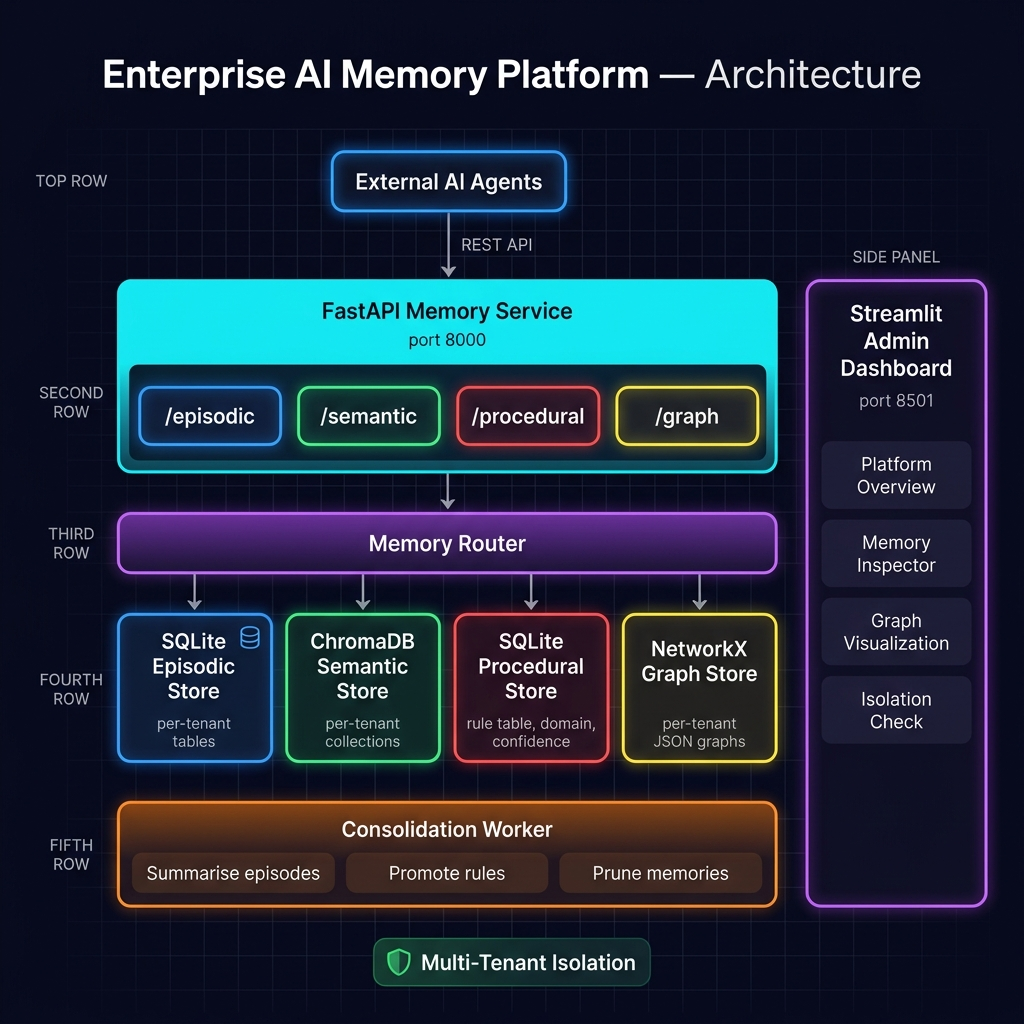
\includegraphics[width=0.85\textwidth]{projects/enterprise_memory_platform/architecture.png}
    \caption{Production Project: Enterprise AI Memory Platform Architecture}
\end{figure}

\subsection{Technical Implementation}
\begin{itemize}[label=\textcolor{secondary}{$\bullet$}]
    \item \textbf{Multi-Tenant Service:} Built using FastAPI, routing memory requests to appropriate stores: SQLite (Episodic \& Procedural), ChromaDB (Semantic), and NetworkX JSON (Knowledge Graph), ensuring strict tenant isolation.
    \item \textbf{Asynchronous Consolidation Worker:} Implemented background tasks that dynamically summarize old episodes, promote high-confidence procedural rules, and prune low-importance memories on a defined schedule.
    \item \textbf{Observability \& Dashboarding:} Features a comprehensive Streamlit Admin Dashboard that visualizes cross-tenant memory states, learning curves, and active procedural rules.
\end{itemize}

\subsection{System Demonstrations}
\begin{figure}[H]
    \centering
    \begin{minipage}{0.48\textwidth}
        \centering
        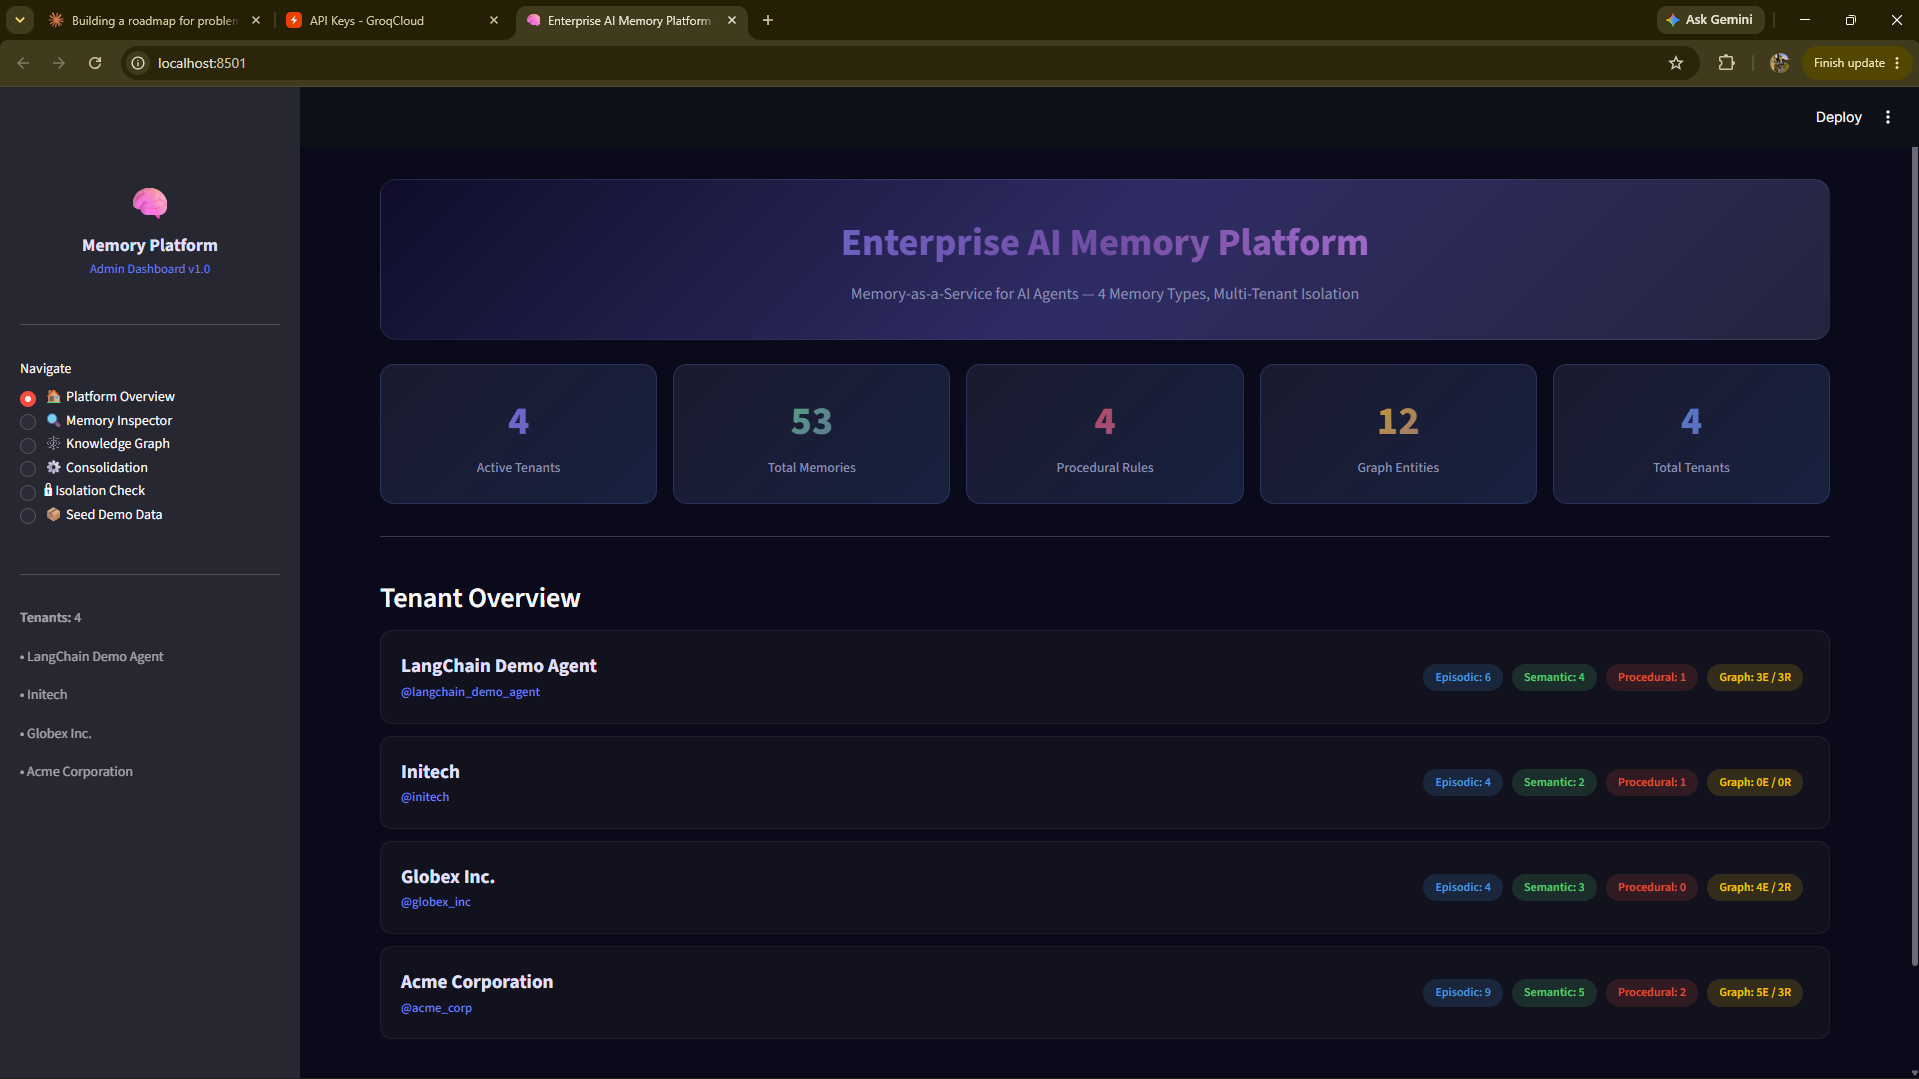
\includegraphics[width=\linewidth, keepaspectratio]{screenshots/Week6/Prod-1.png}
        \caption{Enterprise Memory Platform Dashboard}
    \end{minipage}\hfill
    \begin{minipage}{0.48\textwidth}
        \centering
        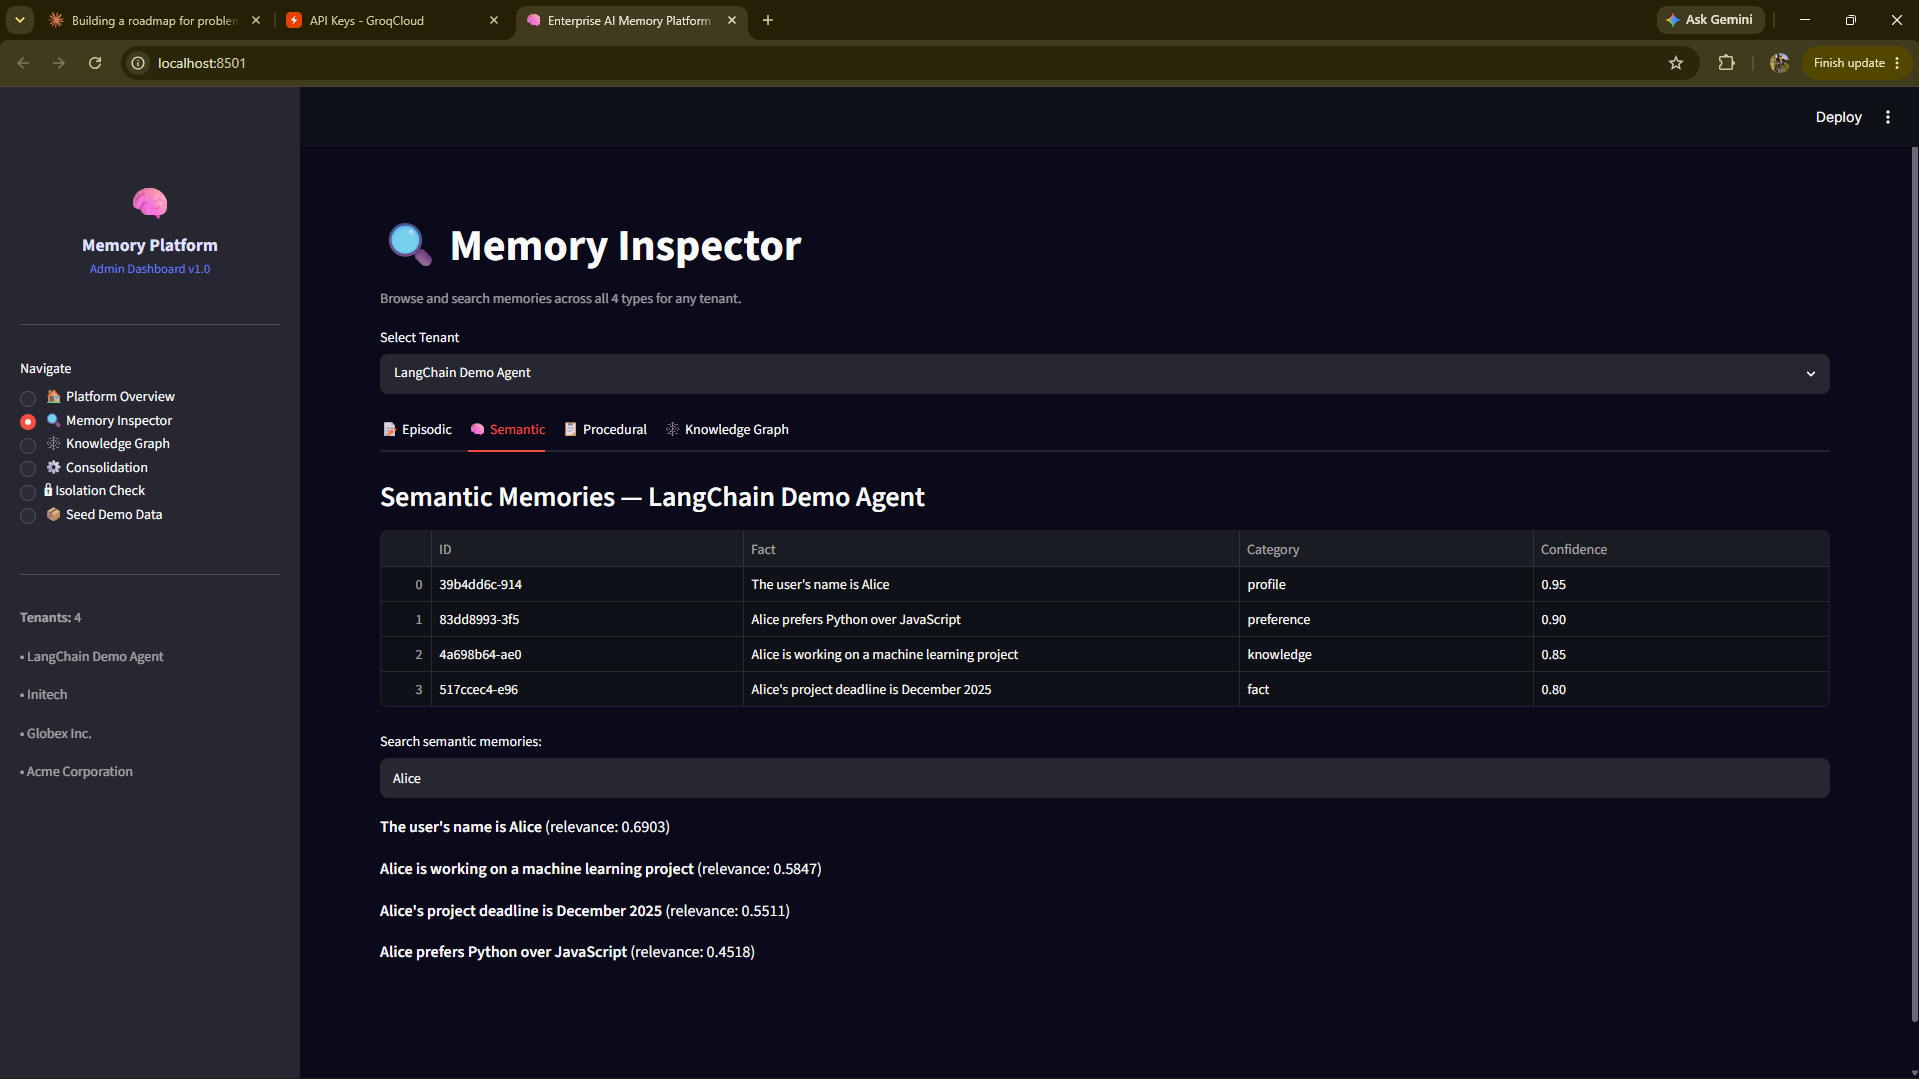
\includegraphics[width=\linewidth, keepaspectratio]{screenshots/Week6/Prod-2.png}
        \caption{Multi-Tenant Memory Inspection}
    \end{minipage}
\end{figure}

\begin{figure}[H]
    \centering
    \begin{minipage}{0.48\textwidth}
        \centering
        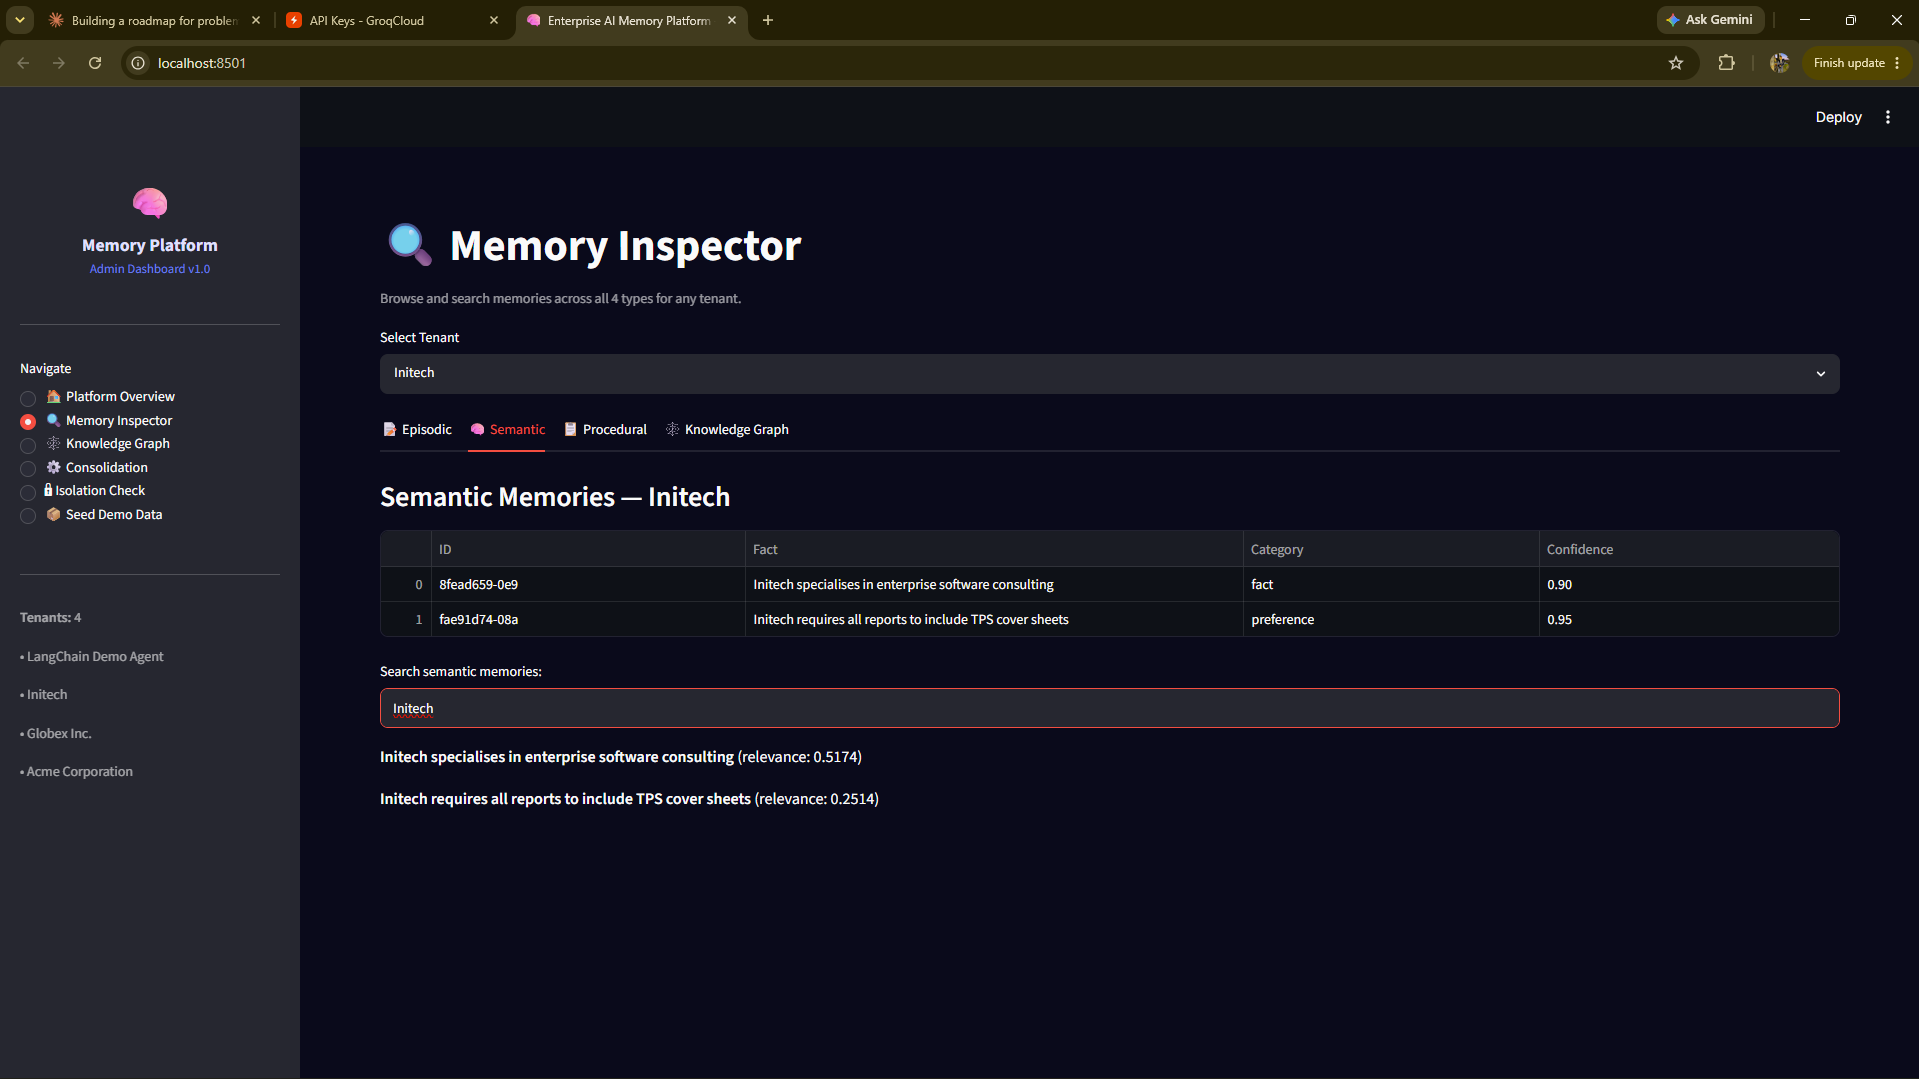
\includegraphics[width=\linewidth, keepaspectratio]{screenshots/Week6/Prod-3.png}
        \caption{Semantic Memory Inspection}
    \end{minipage}\hfill
    \begin{minipage}{0.48\textwidth}
        \centering
        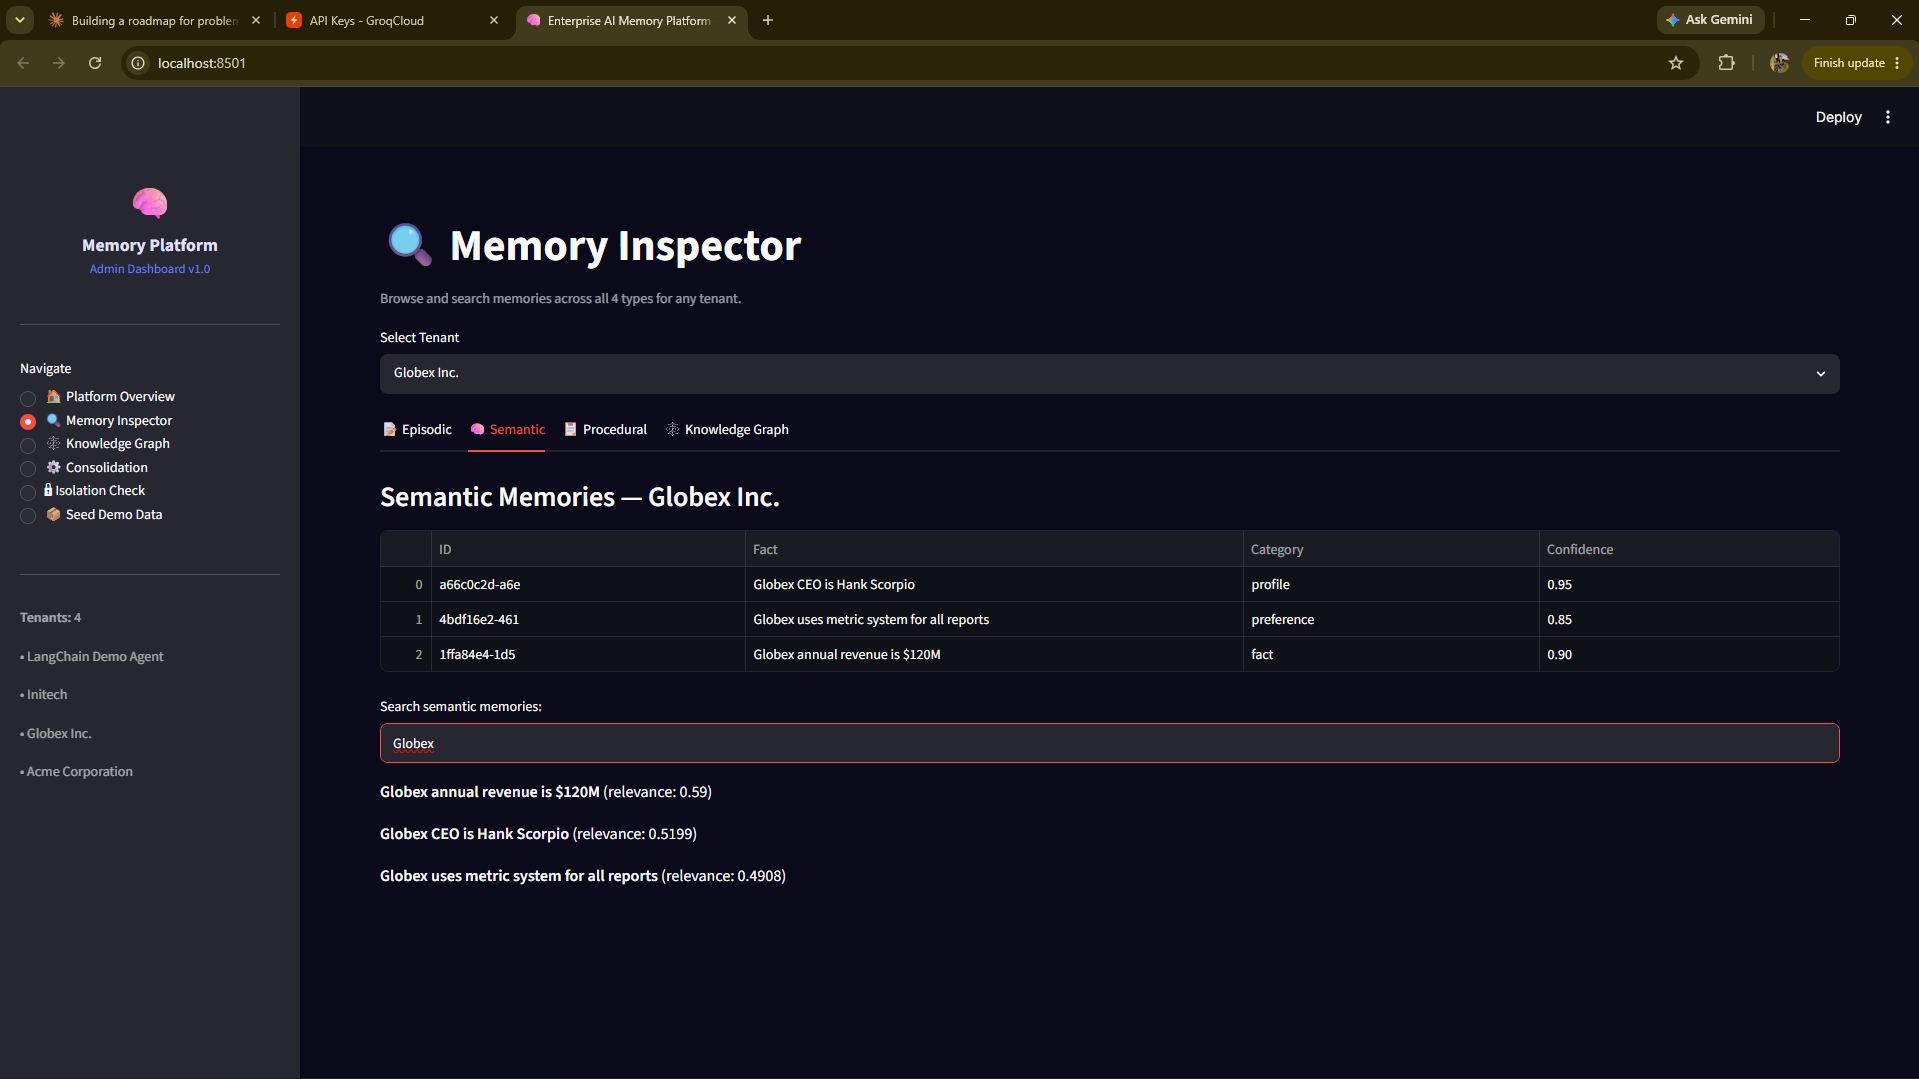
\includegraphics[width=\linewidth, keepaspectratio]{screenshots/Week6/Prod-4.png}
        \caption{Globex Memory Inspection}
    \end{minipage}
\end{figure}

\begin{figure}[H]
    \centering
    \begin{minipage}{0.48\textwidth}
        \centering
        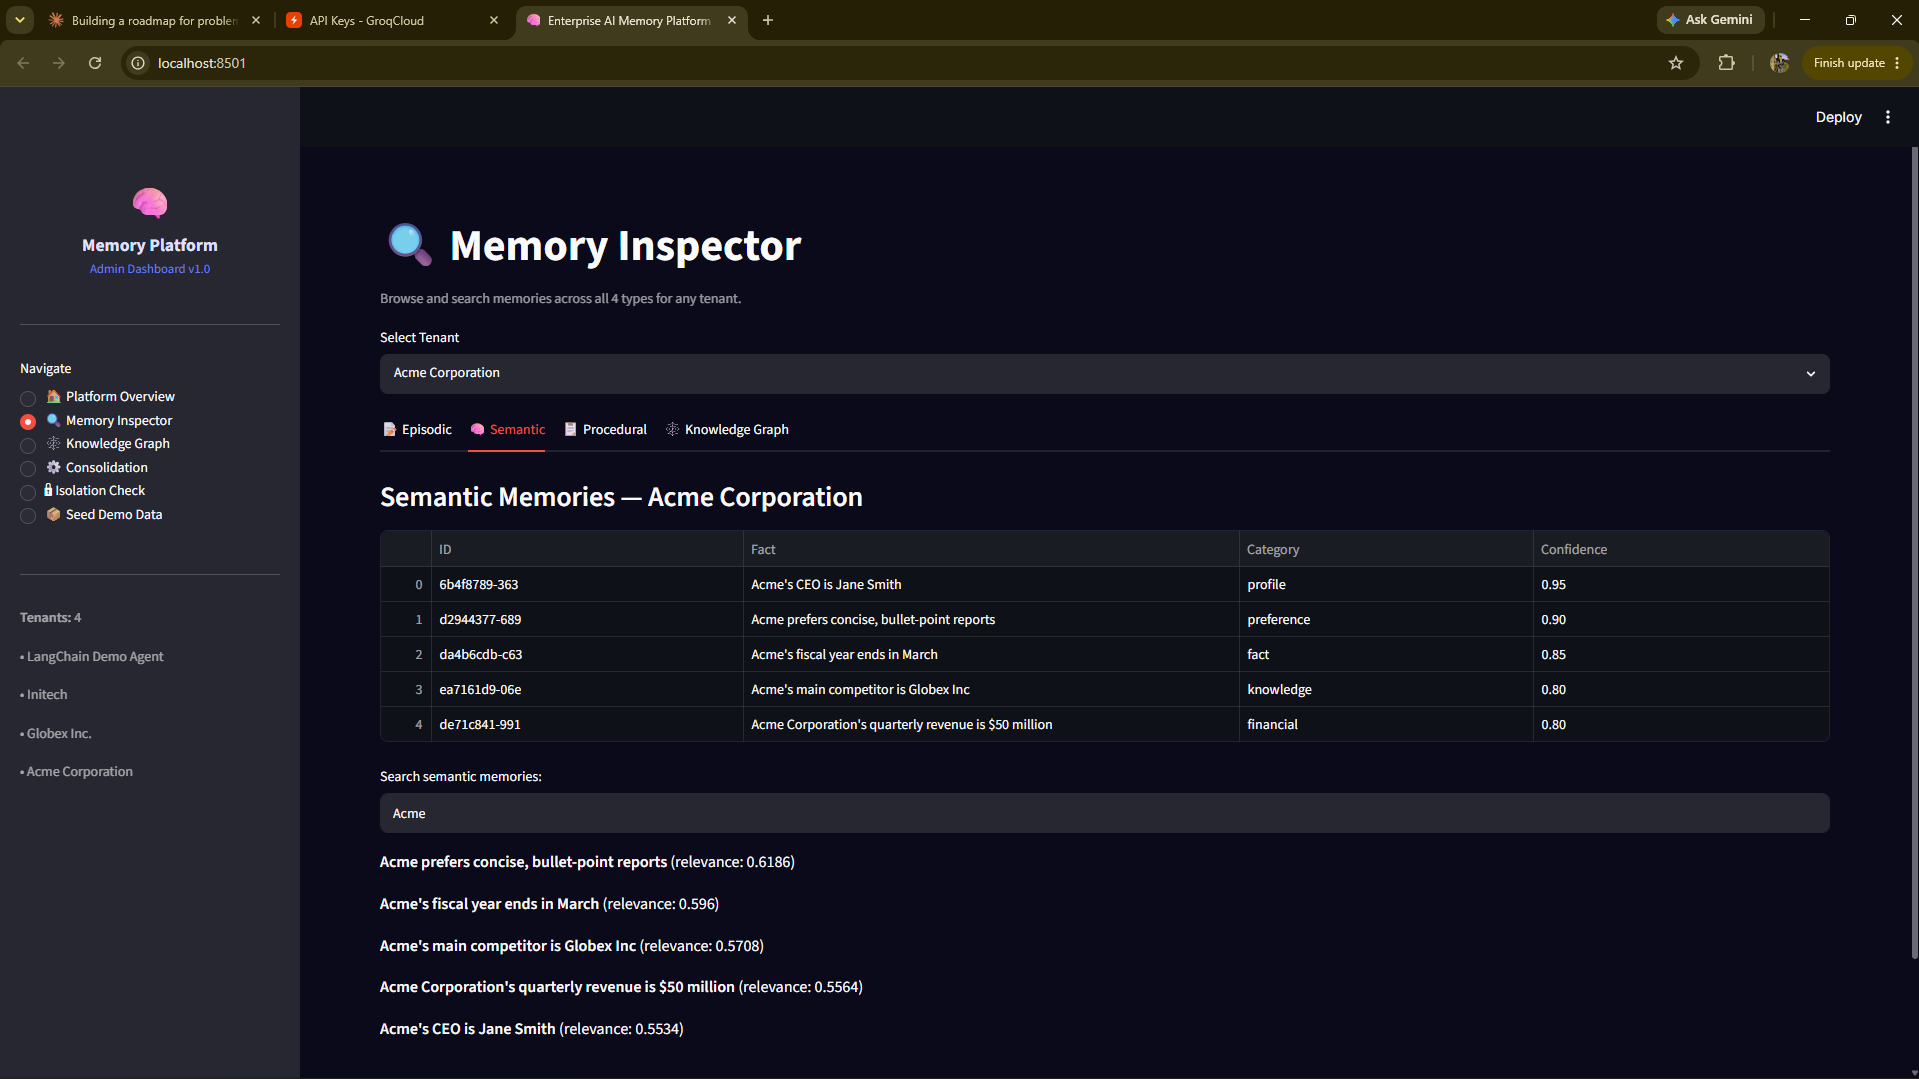
\includegraphics[width=\linewidth, keepaspectratio]{screenshots/Week6/Prod-5.png}
        \caption{ChromaDB Collection Viewer}
    \end{minipage}\hfill
    \begin{minipage}{0.48\textwidth}
        \centering
        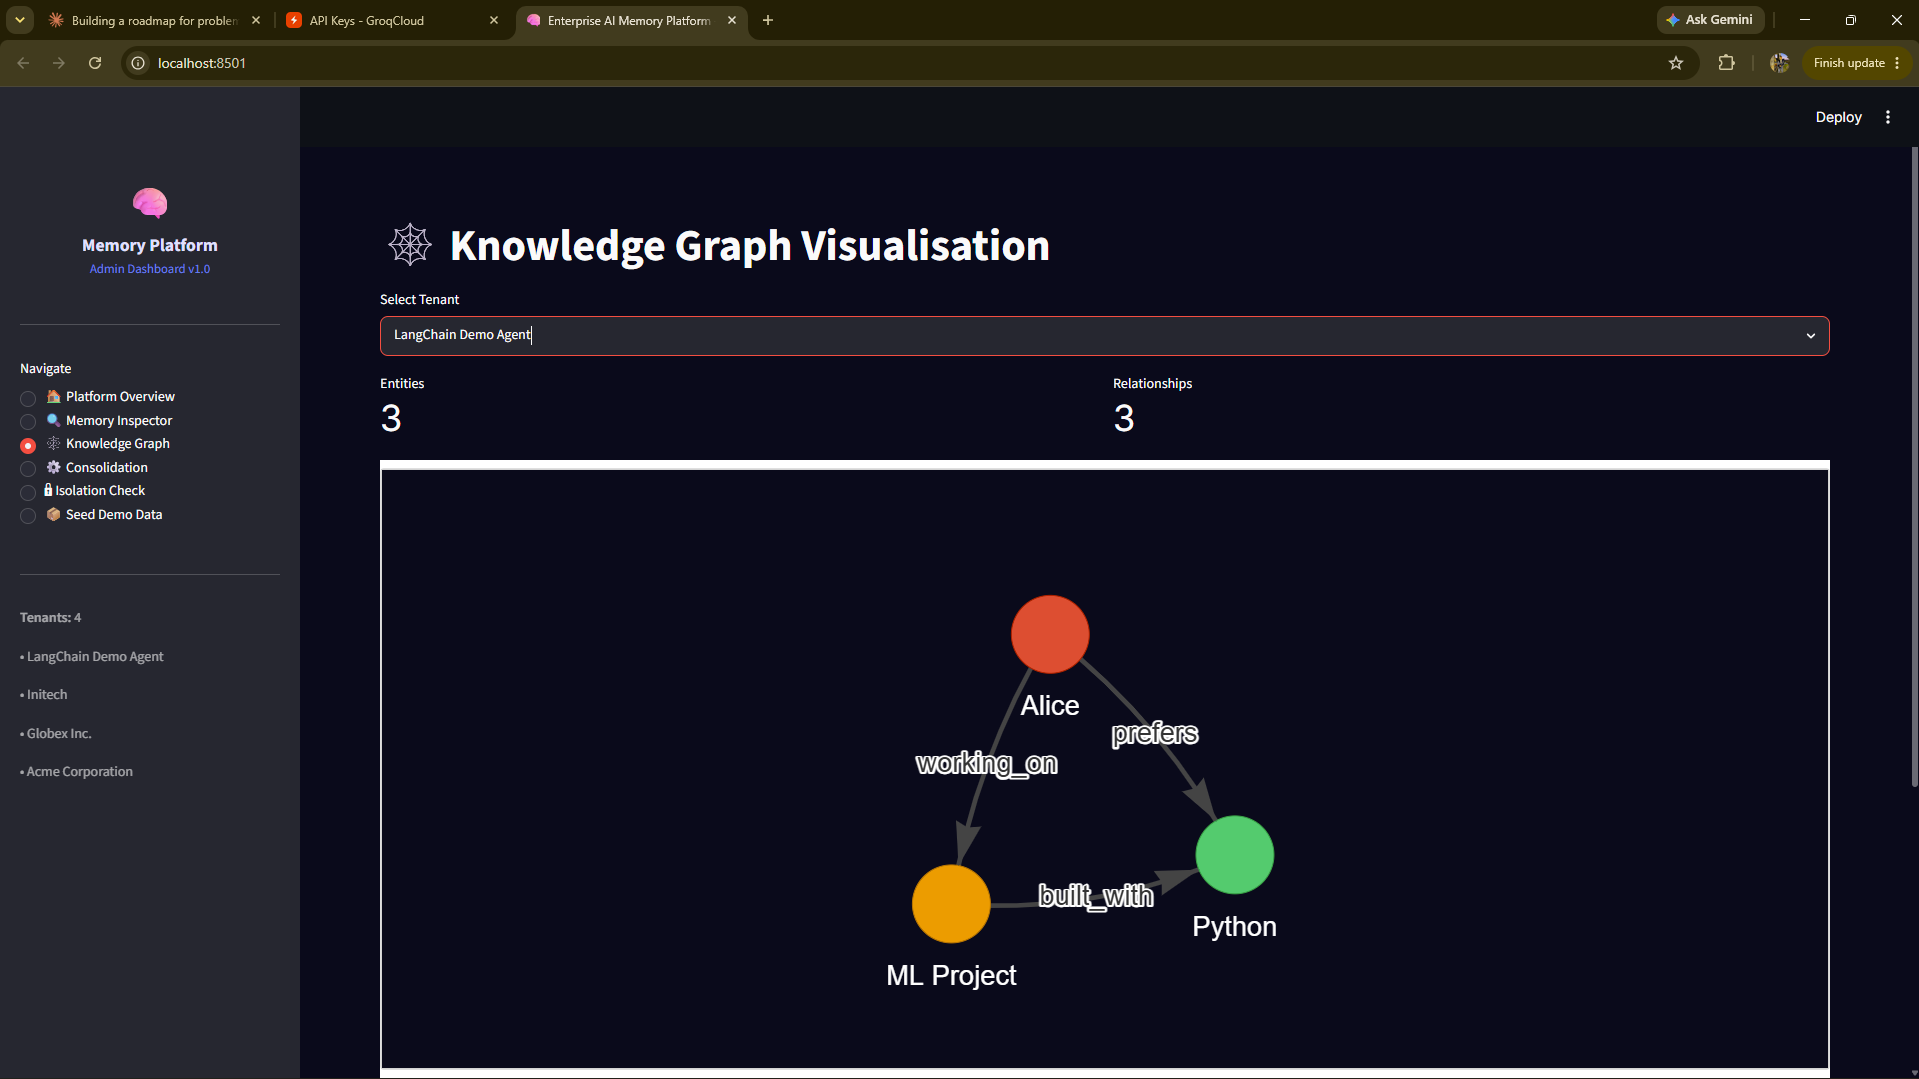
\includegraphics[width=\linewidth, keepaspectratio]{screenshots/Week6/Prod-6.png}
        \caption{Knowledge Graph Visualisation}
    \end{minipage}
\end{figure}

\begin{figure}[H]
    \centering
    \begin{minipage}{0.48\textwidth}
        \centering
        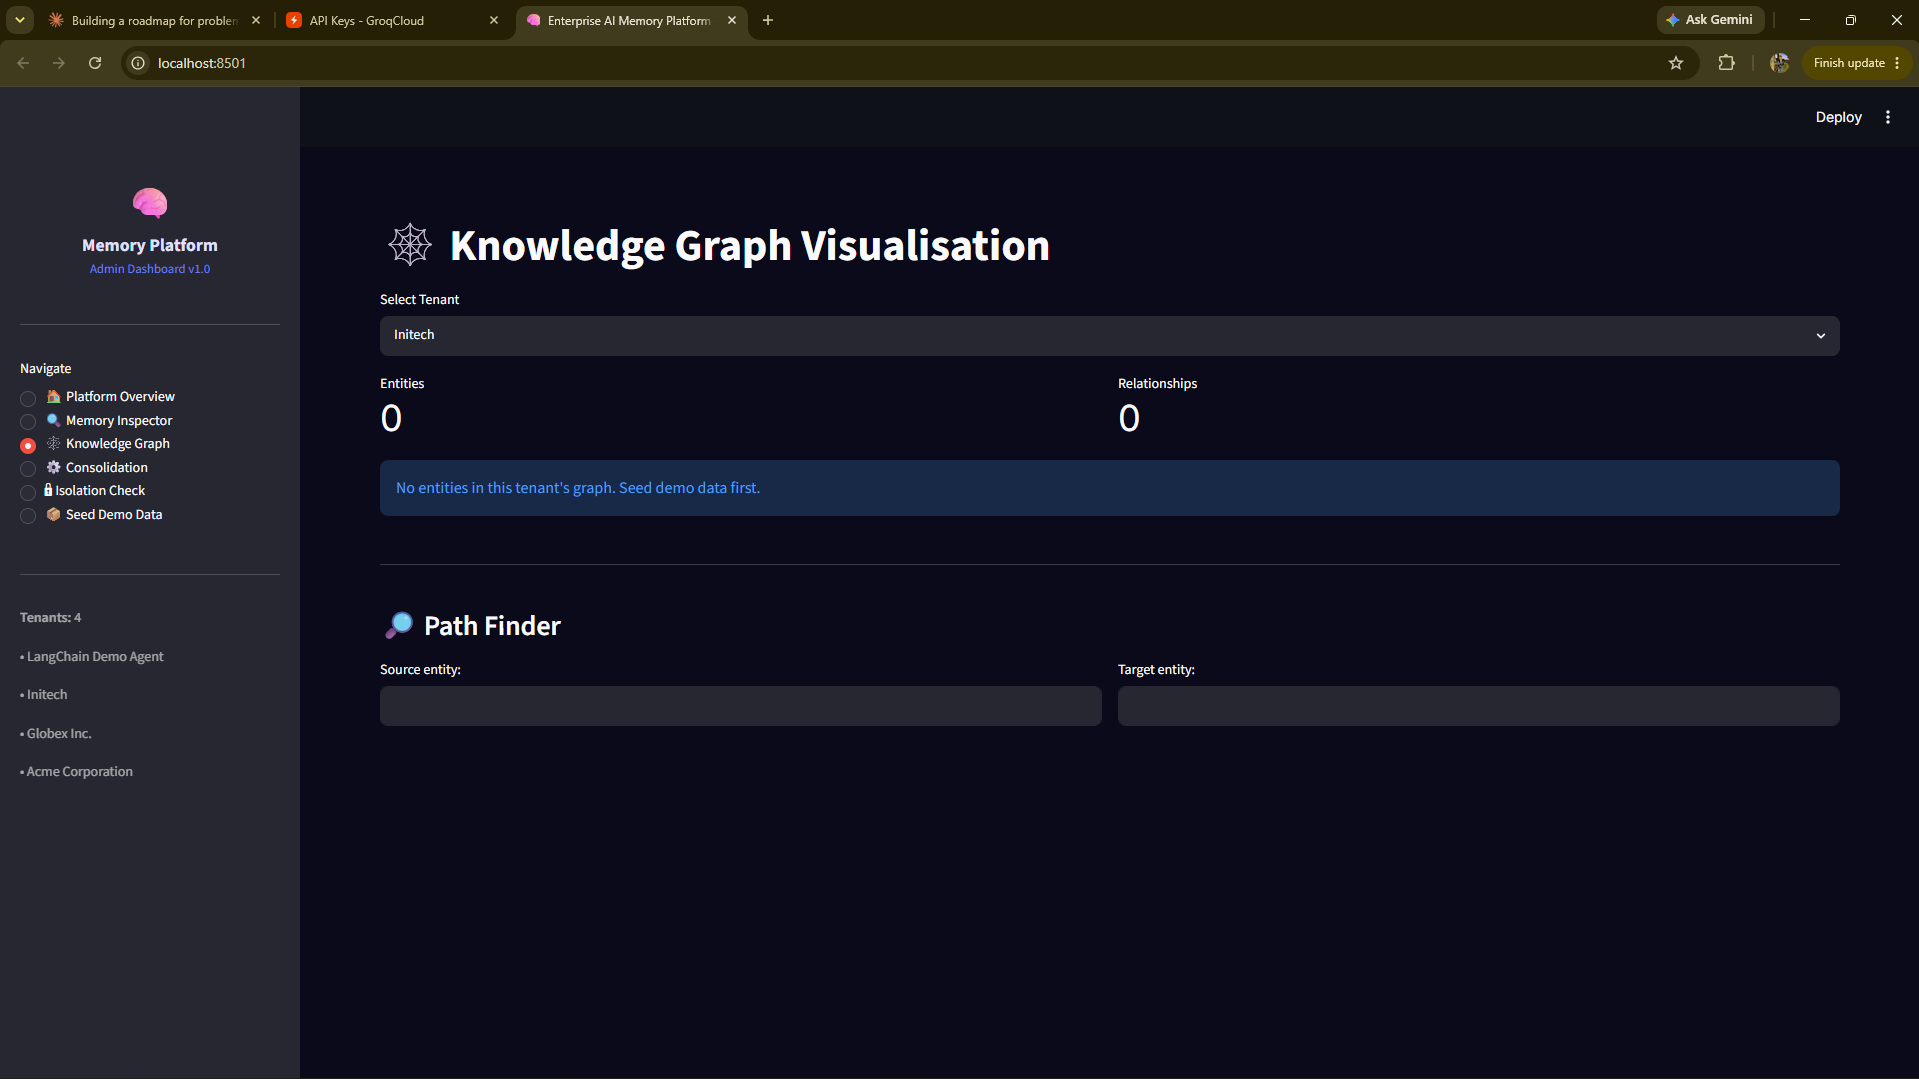
\includegraphics[width=\linewidth, keepaspectratio]{screenshots/Week6/Prod-7.png}
        \caption{Knowledge Graph State}
    \end{minipage}\hfill
    \begin{minipage}{0.48\textwidth}
        \centering
        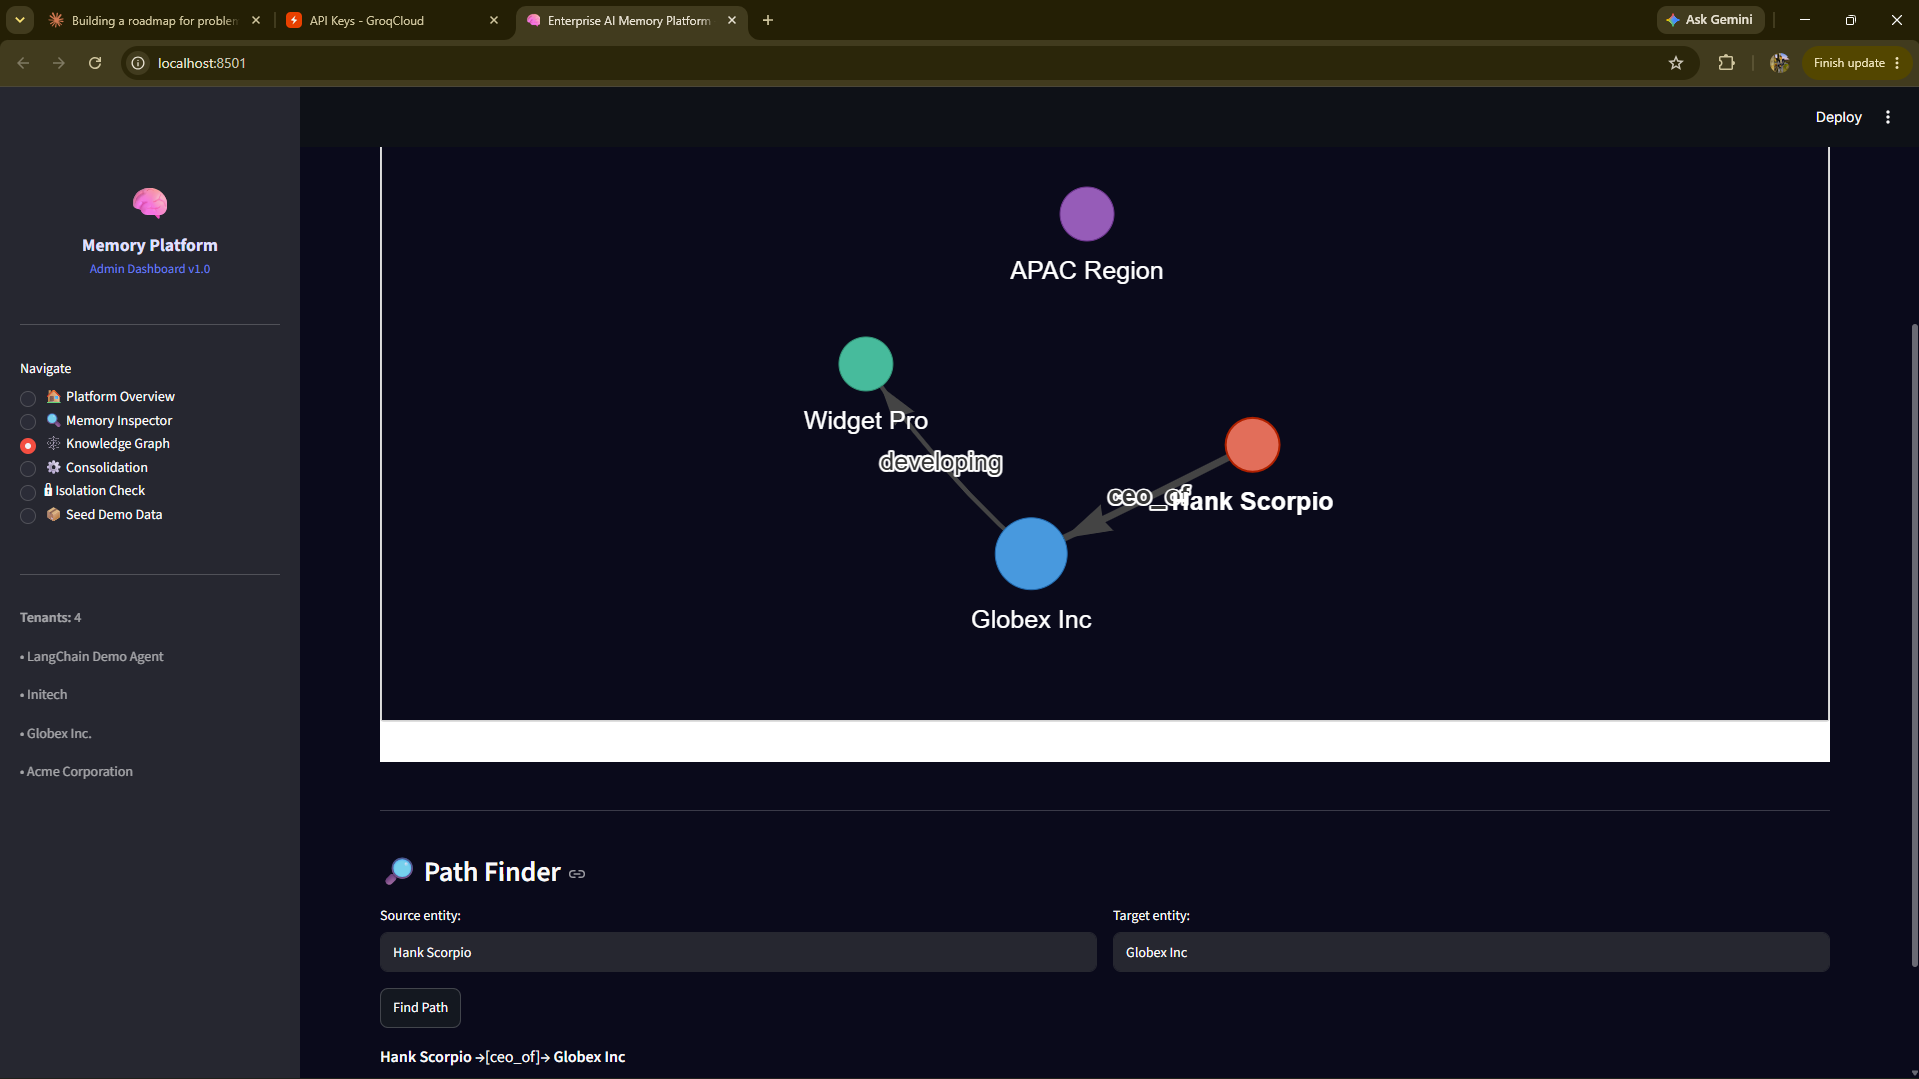
\includegraphics[width=\linewidth, keepaspectratio]{screenshots/Week6/Prod-8.png}
        \caption{Memory Router Decision Trace}
    \end{minipage}
\end{figure}

\begin{figure}[H]
    \centering
    \begin{minipage}{0.48\textwidth}
        \centering
        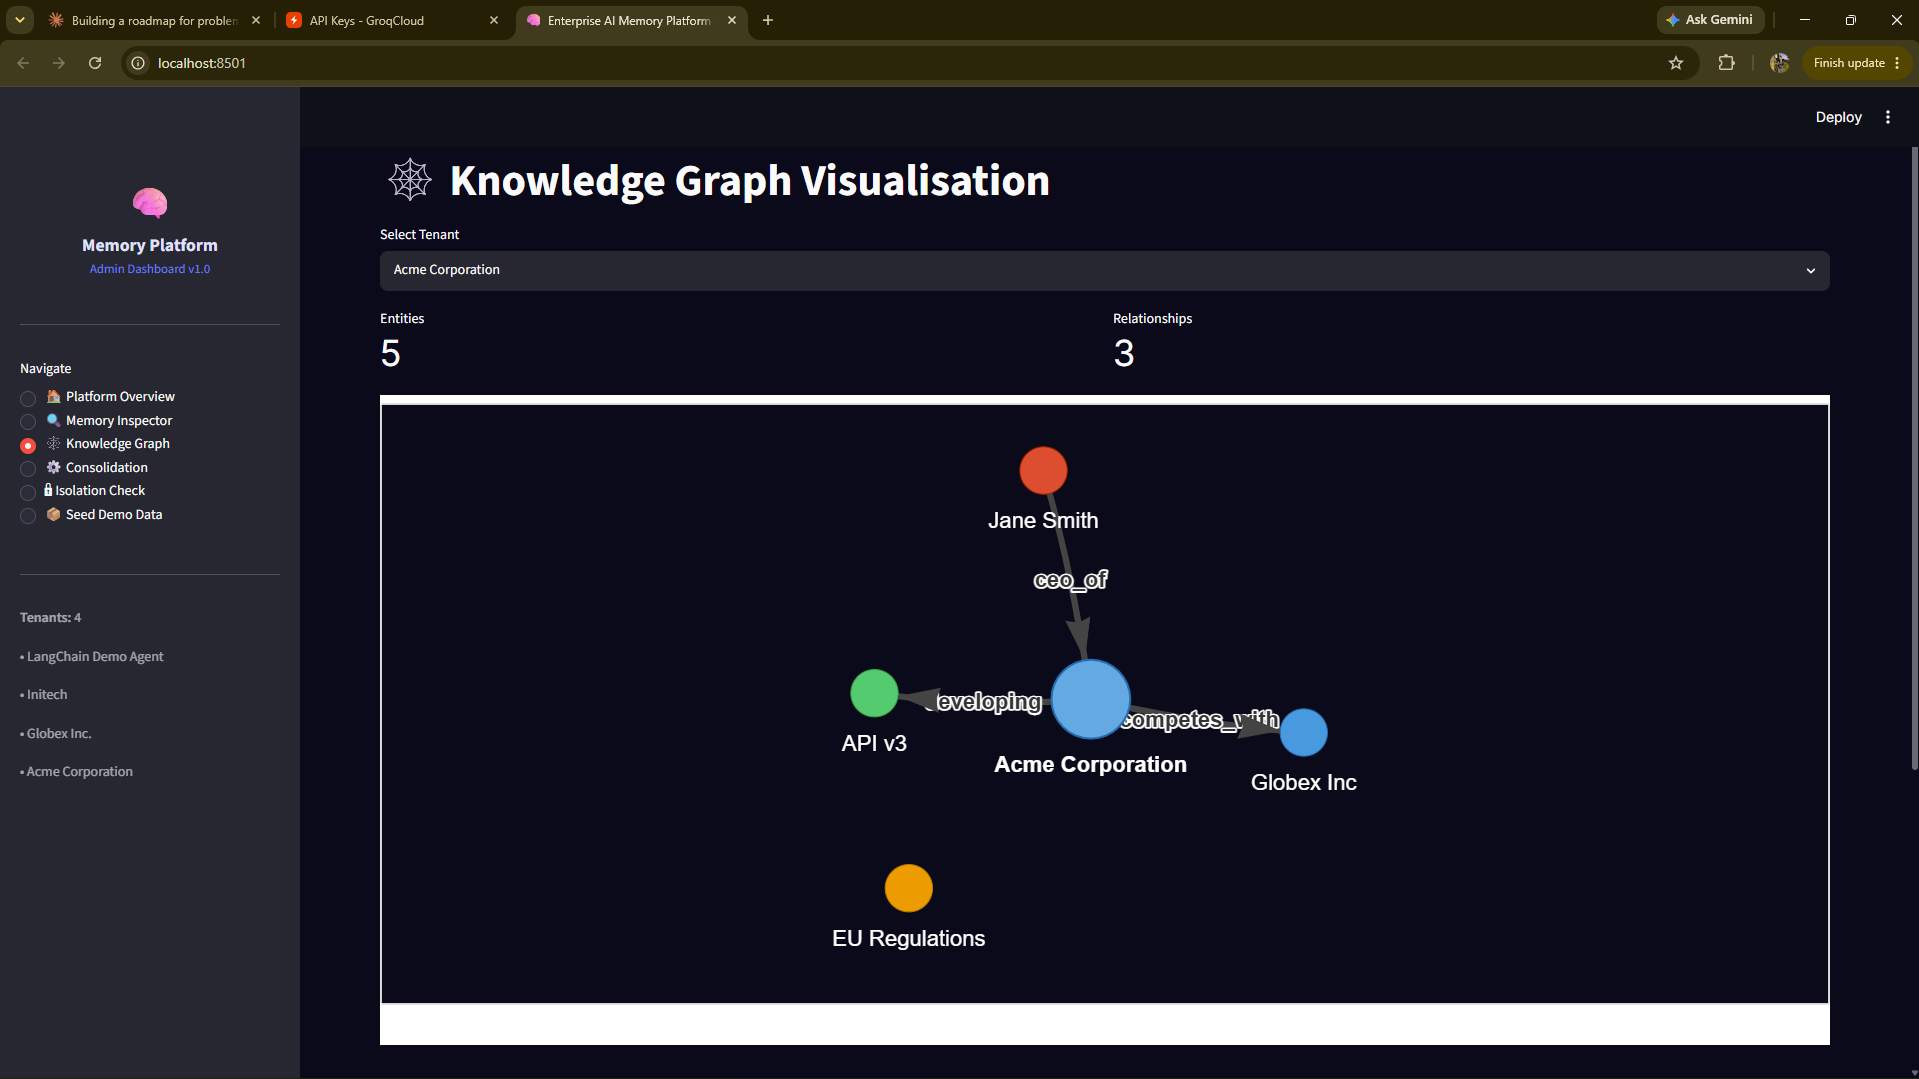
\includegraphics[width=\linewidth, keepaspectratio]{screenshots/Week6/Prod-9.png}
        \caption{Acme Corporation Graph}
    \end{minipage}\hfill
    \begin{minipage}{0.48\textwidth}
        \centering
        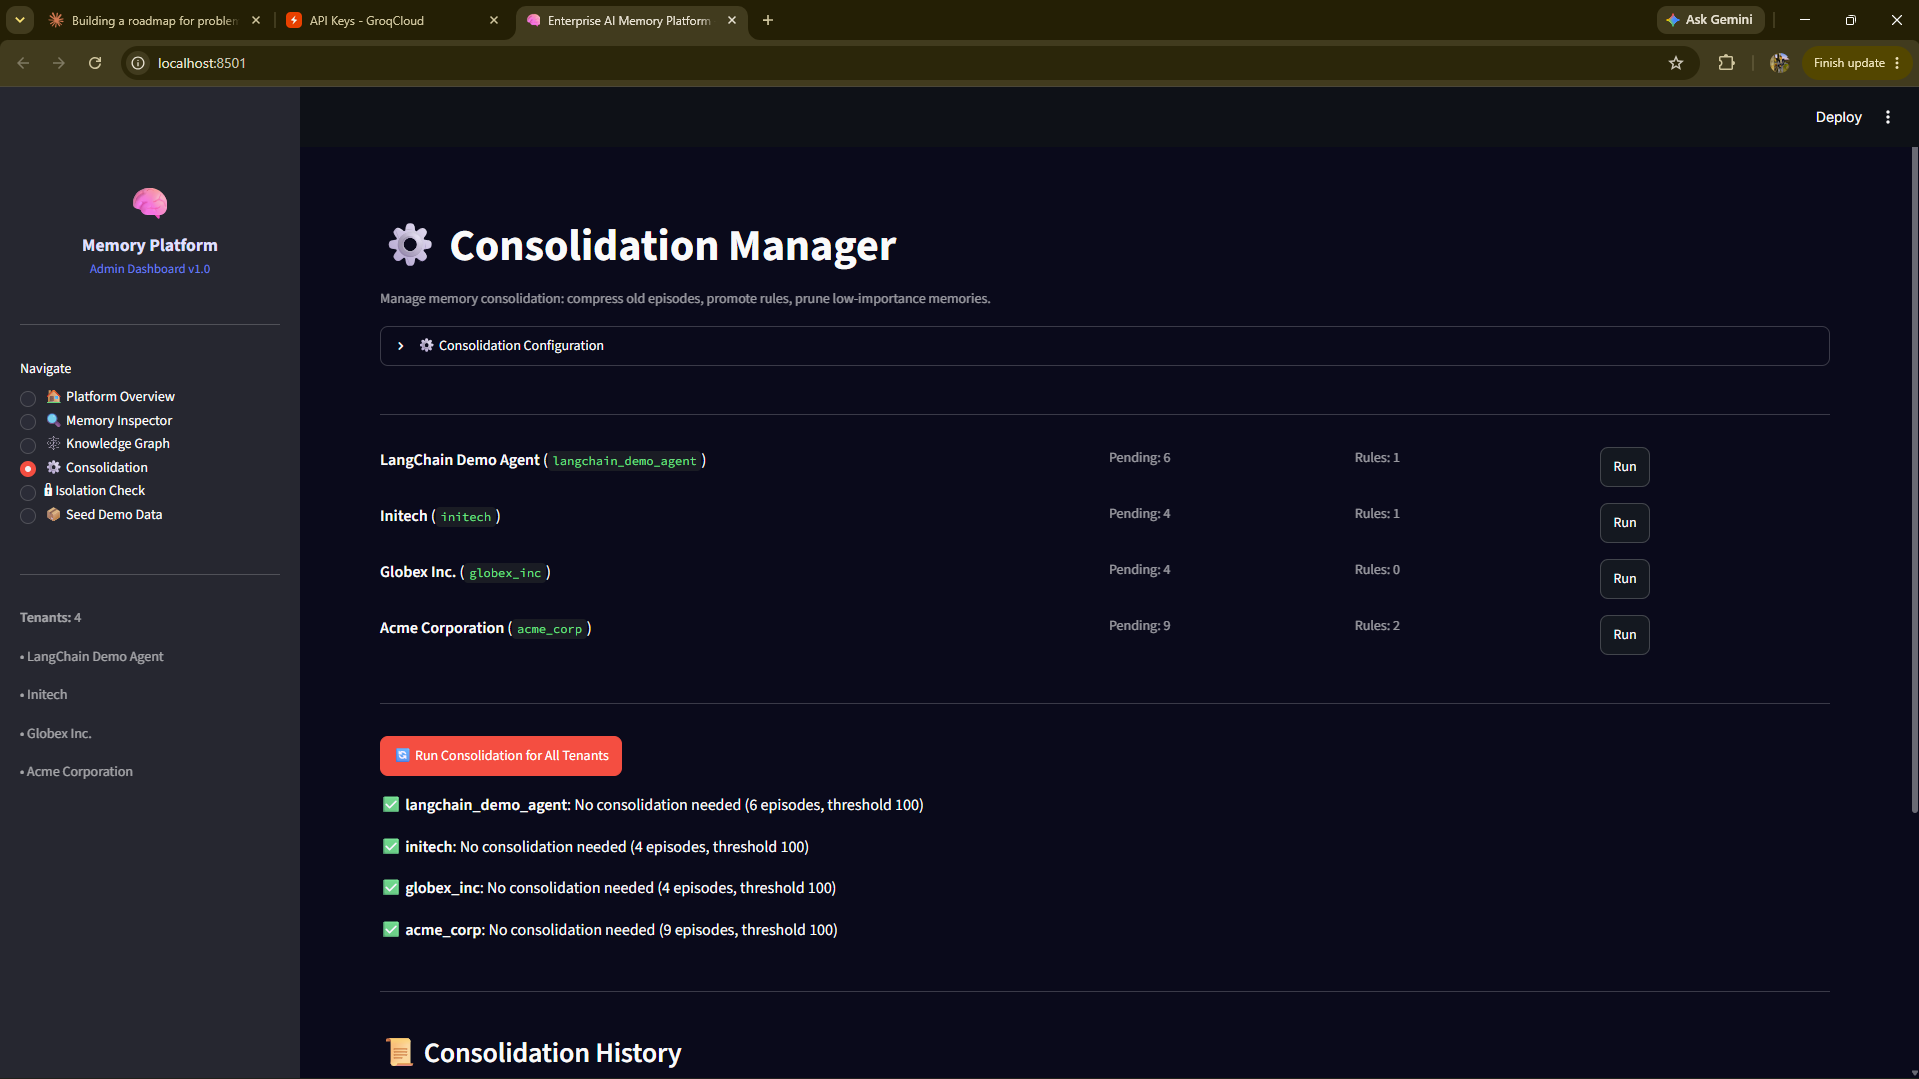
\includegraphics[width=\linewidth, keepaspectratio]{screenshots/Week6/Prod-10.png}
        \caption{Consolidation Worker}
    \end{minipage}
\end{figure}

\begin{figure}[H]
    \centering
    \begin{minipage}{0.48\textwidth}
        \centering
        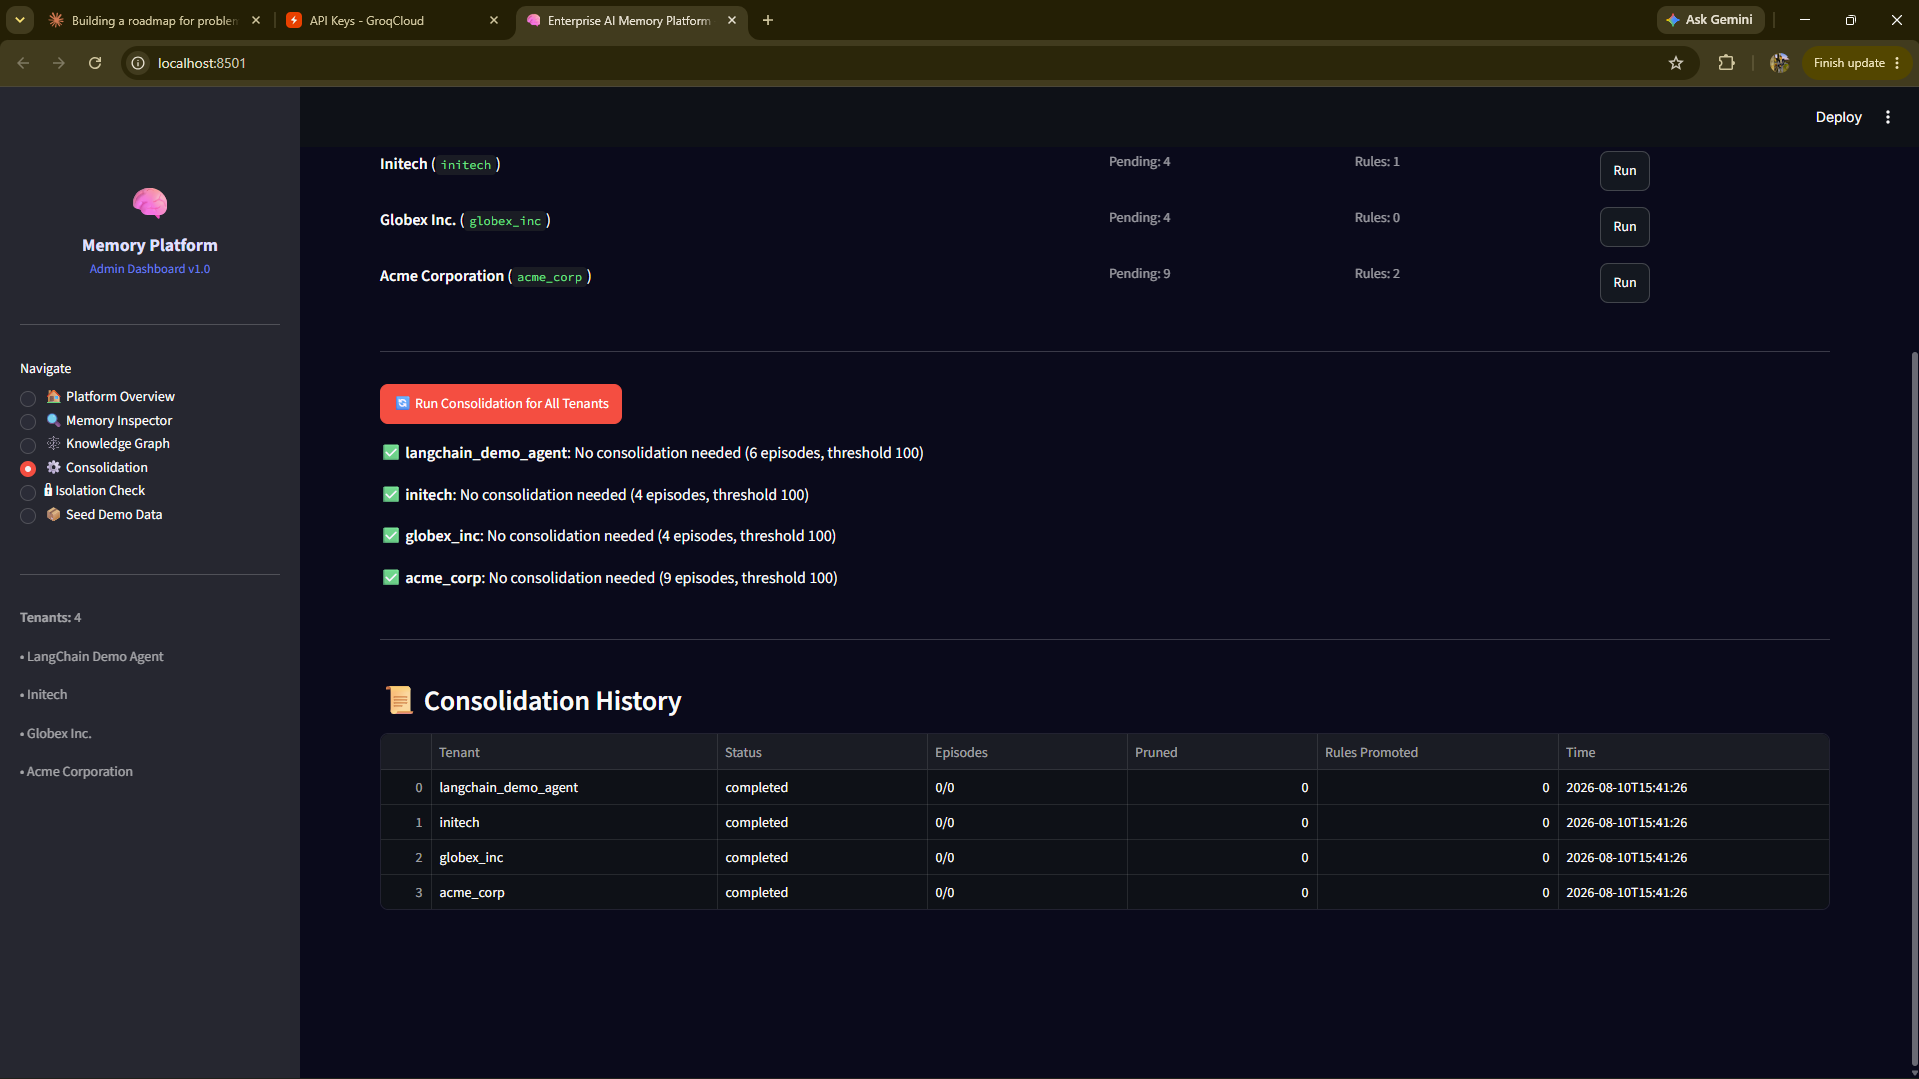
\includegraphics[width=\linewidth, keepaspectratio]{screenshots/Week6/Prod-11.png}
        \caption{Tenants Consolidation History}
    \end{minipage}\hfill
    \begin{minipage}{0.48\textwidth}
        \centering
        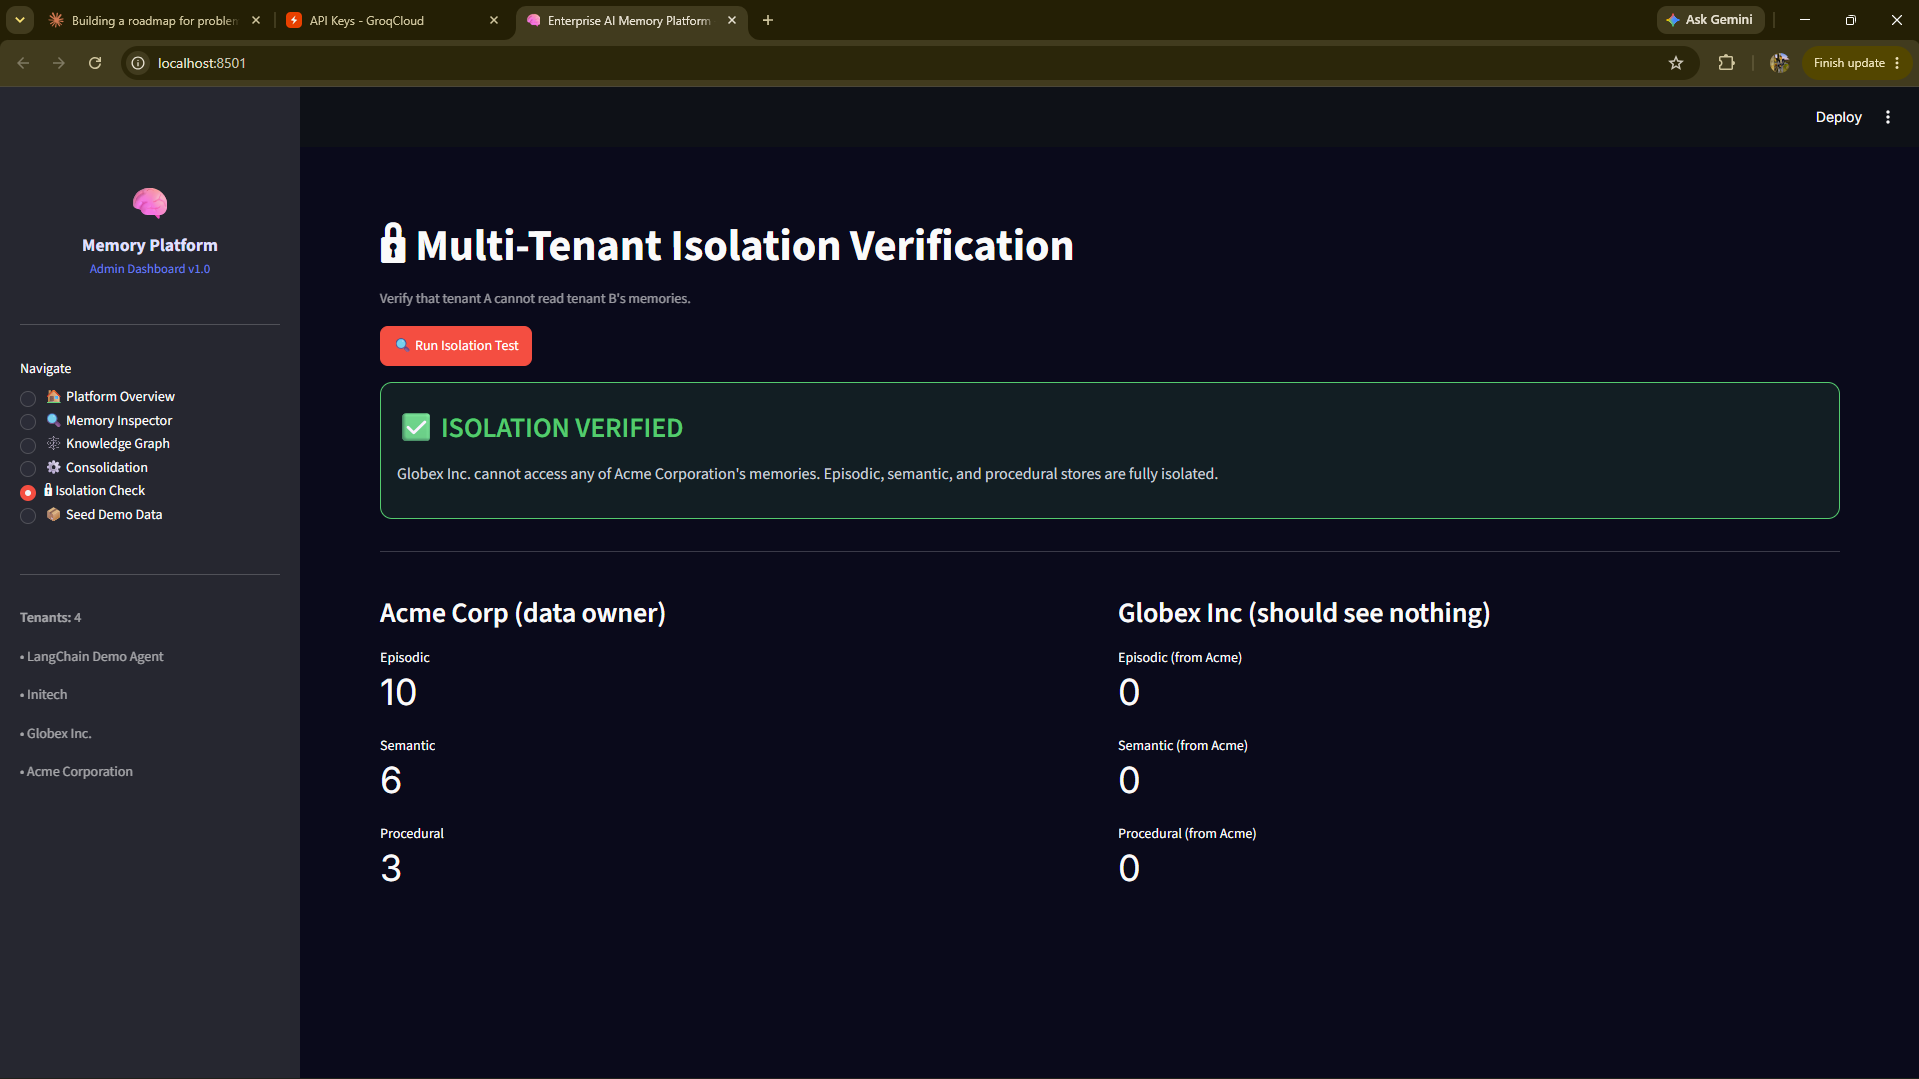
\includegraphics[width=\linewidth, keepaspectratio]{screenshots/Week6/Prod-12.png}
        \caption{Multi-Tenant Verification}
    \end{minipage}
\end{figure}

\newpage

% --- Section 4: Intermediate Project ---
\section{Intermediate Project: Procedural Memory \& Self-Improving Agent}

\begin{tcolorbox}[colback=accent, colframe=primary, title=\textbf{Architectural Overview}, boxrule=1pt]
An advanced autonomous agent engineered to learn from its own mistakes over time. It utilizes procedural memory to extract specific corrections (rules) made by users, stores them securely, and applies semantic retrieval to ensure identical errors are permanently avoided.
\end{tcolorbox}

\begin{figure}[H]
    \centering
    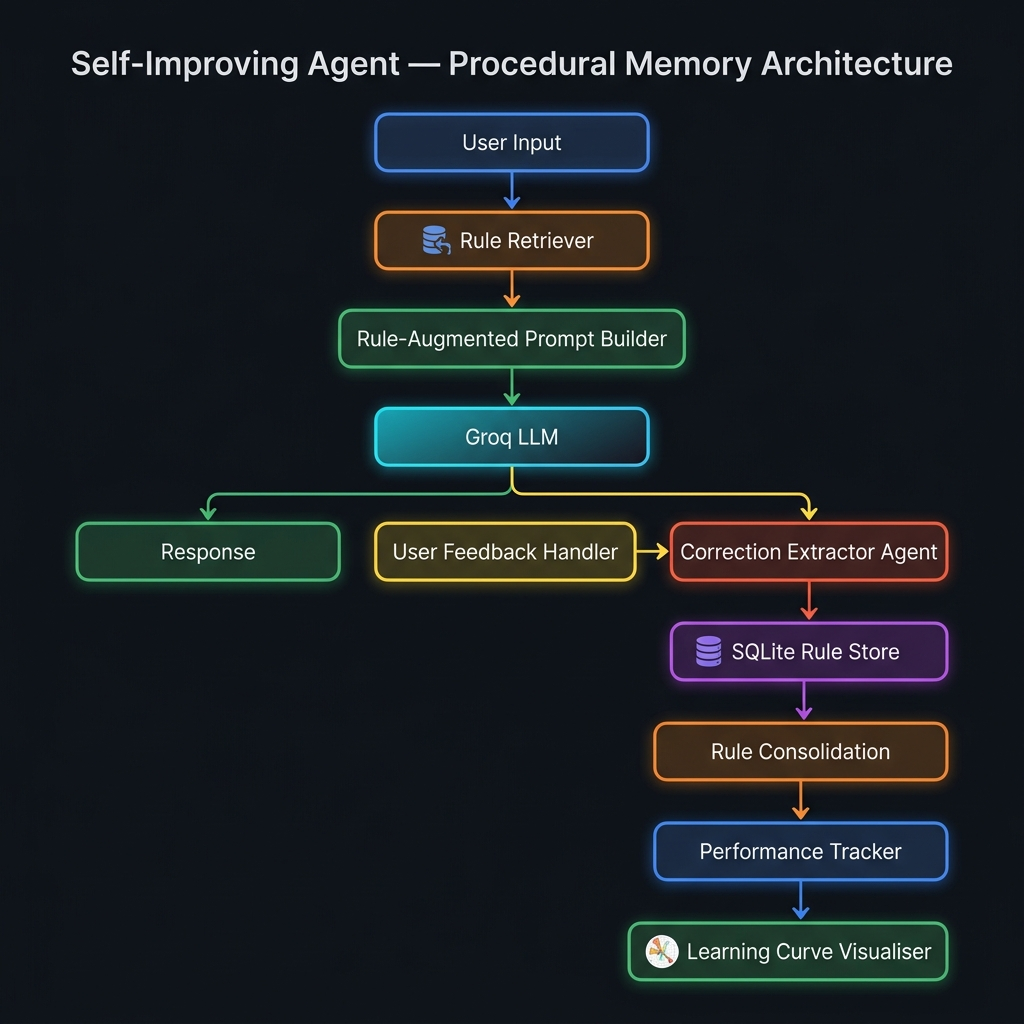
\includegraphics[width=0.85\textwidth]{projects/self_improving_agent/architecture.png}
    \caption{Intermediate Project: Procedural Memory \& Self-Improving Agent Architecture}
\end{figure}

\subsection{Technical Implementation}
\begin{itemize}[label=\textcolor{secondary}{$\bullet$}]
    \item \textbf{Dynamic Rule Construction:} Constructed a Correction Extractor Agent that identifies mistakes, synthesizes actionable rules, and commits them to a SQLite procedural store.
    \item \textbf{Rule-Augmented Generation:} Integrated a mechanism where the Rule Retriever fetches contextually relevant instructions at query time to formulate a fortified, error-free prompt before generating an answer.
    \item \textbf{Measurable Improvement:} Deployed performance trackers and visualization pipelines using matplotlib to dynamically chart the learning curve, proving a measurable decrease in error rate over 20+ interactions.
\end{itemize}

\subsection{System Demonstrations}
\begin{figure}[H]
    \centering
    \begin{minipage}{0.48\textwidth}
        \centering
        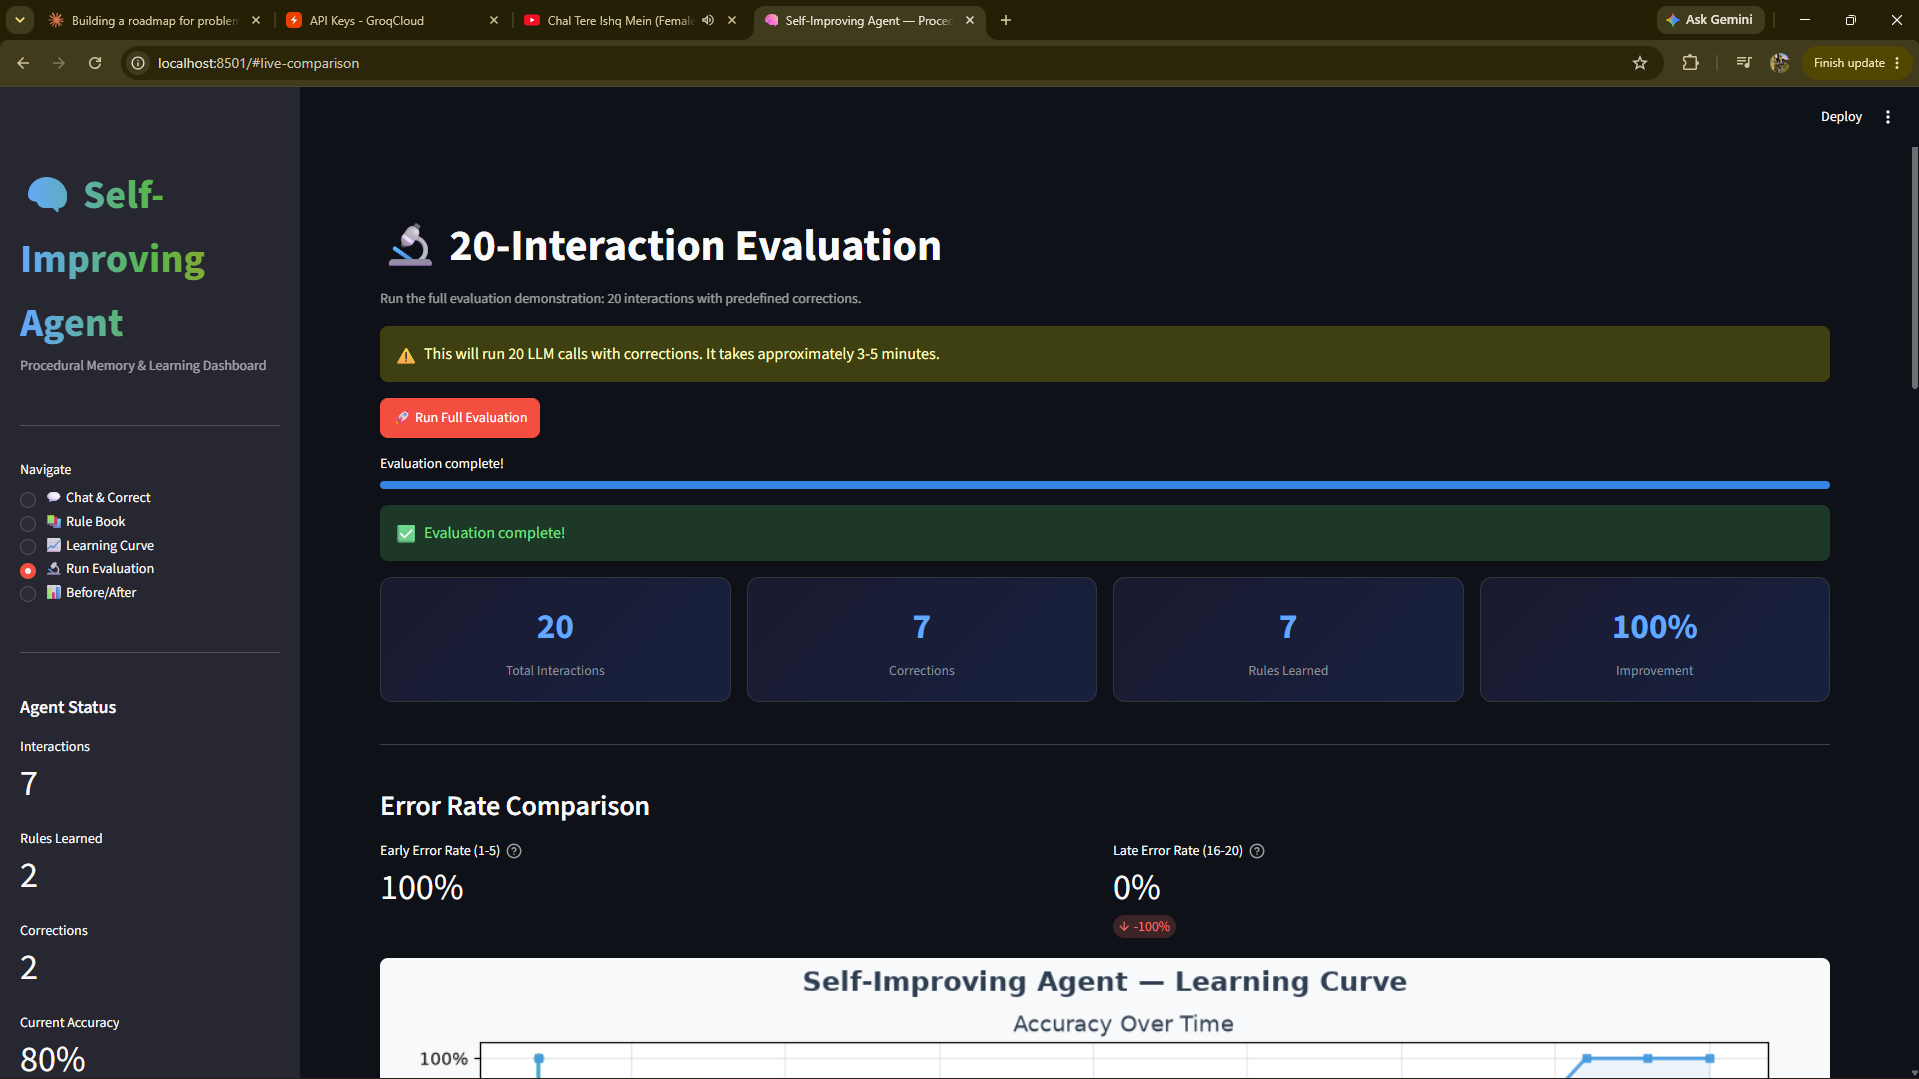
\includegraphics[width=\linewidth, keepaspectratio]{screenshots/Week6/Inter-1.png}
        \caption{20-Interaction Evaluation}
    \end{minipage}\hfill
    \begin{minipage}{0.48\textwidth}
        \centering
        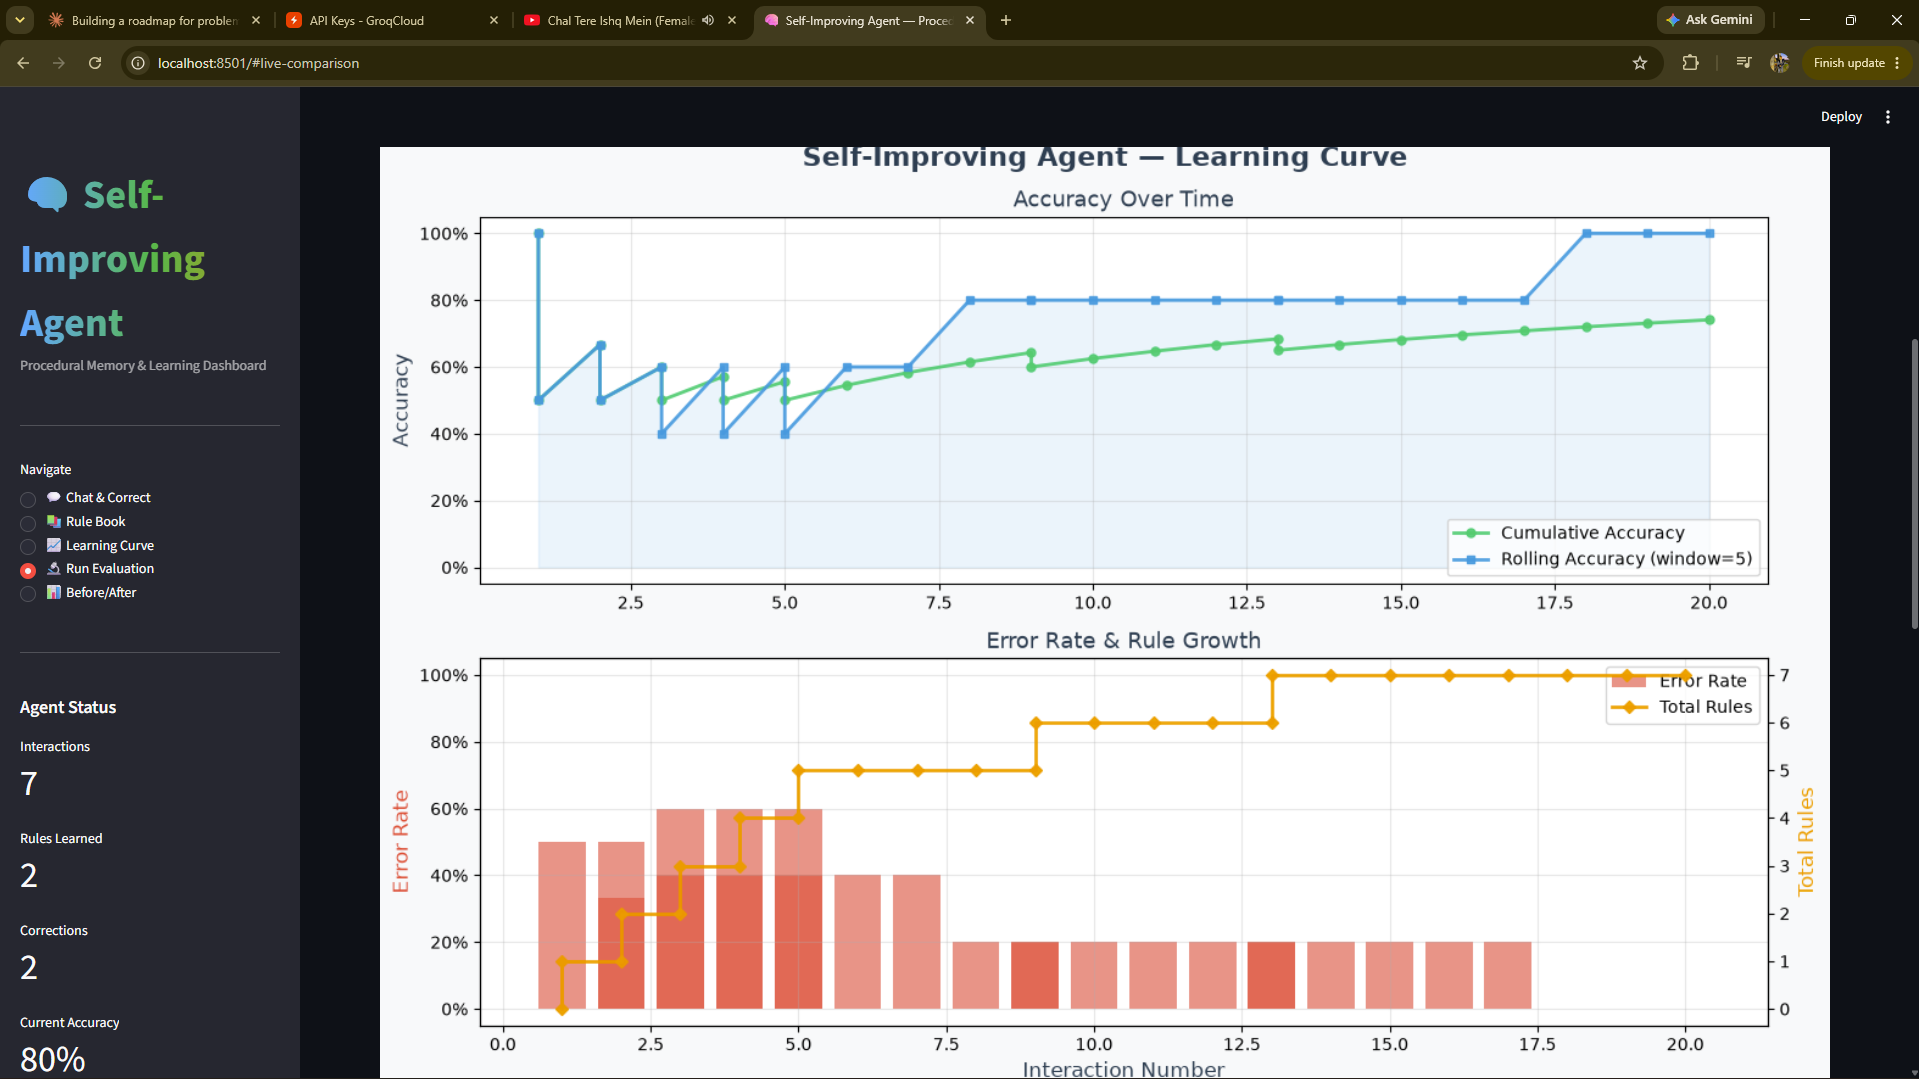
\includegraphics[width=\linewidth, keepaspectratio]{screenshots/Week6/Inter-2.png}
        \caption{Agent Learning Curve}
    \end{minipage}
\end{figure}

\begin{figure}[H]
    \centering
    \begin{minipage}{0.48\textwidth}
        \centering
        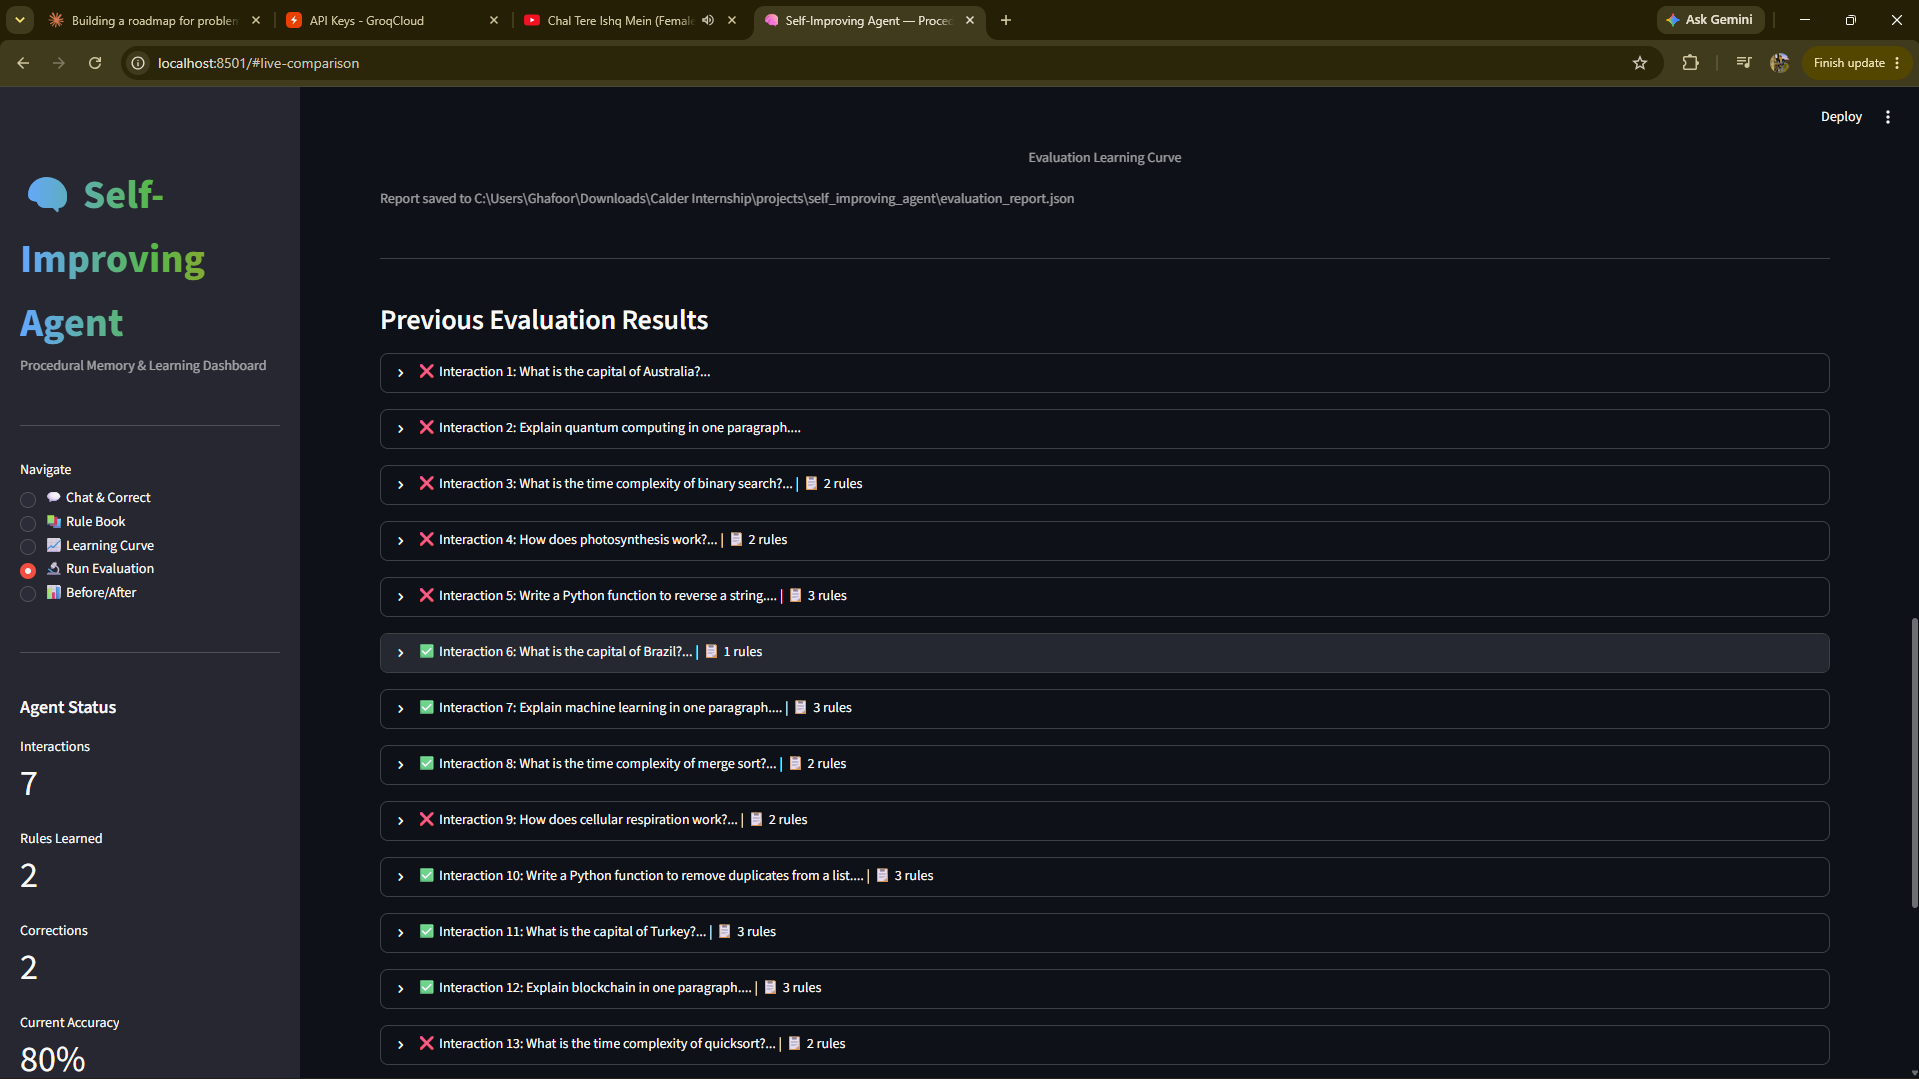
\includegraphics[width=\linewidth, keepaspectratio]{screenshots/Week6/Inter-3.png}
        \caption{Run Evaluation Results}
    \end{minipage}\hfill
    \begin{minipage}{0.48\textwidth}
        \centering
        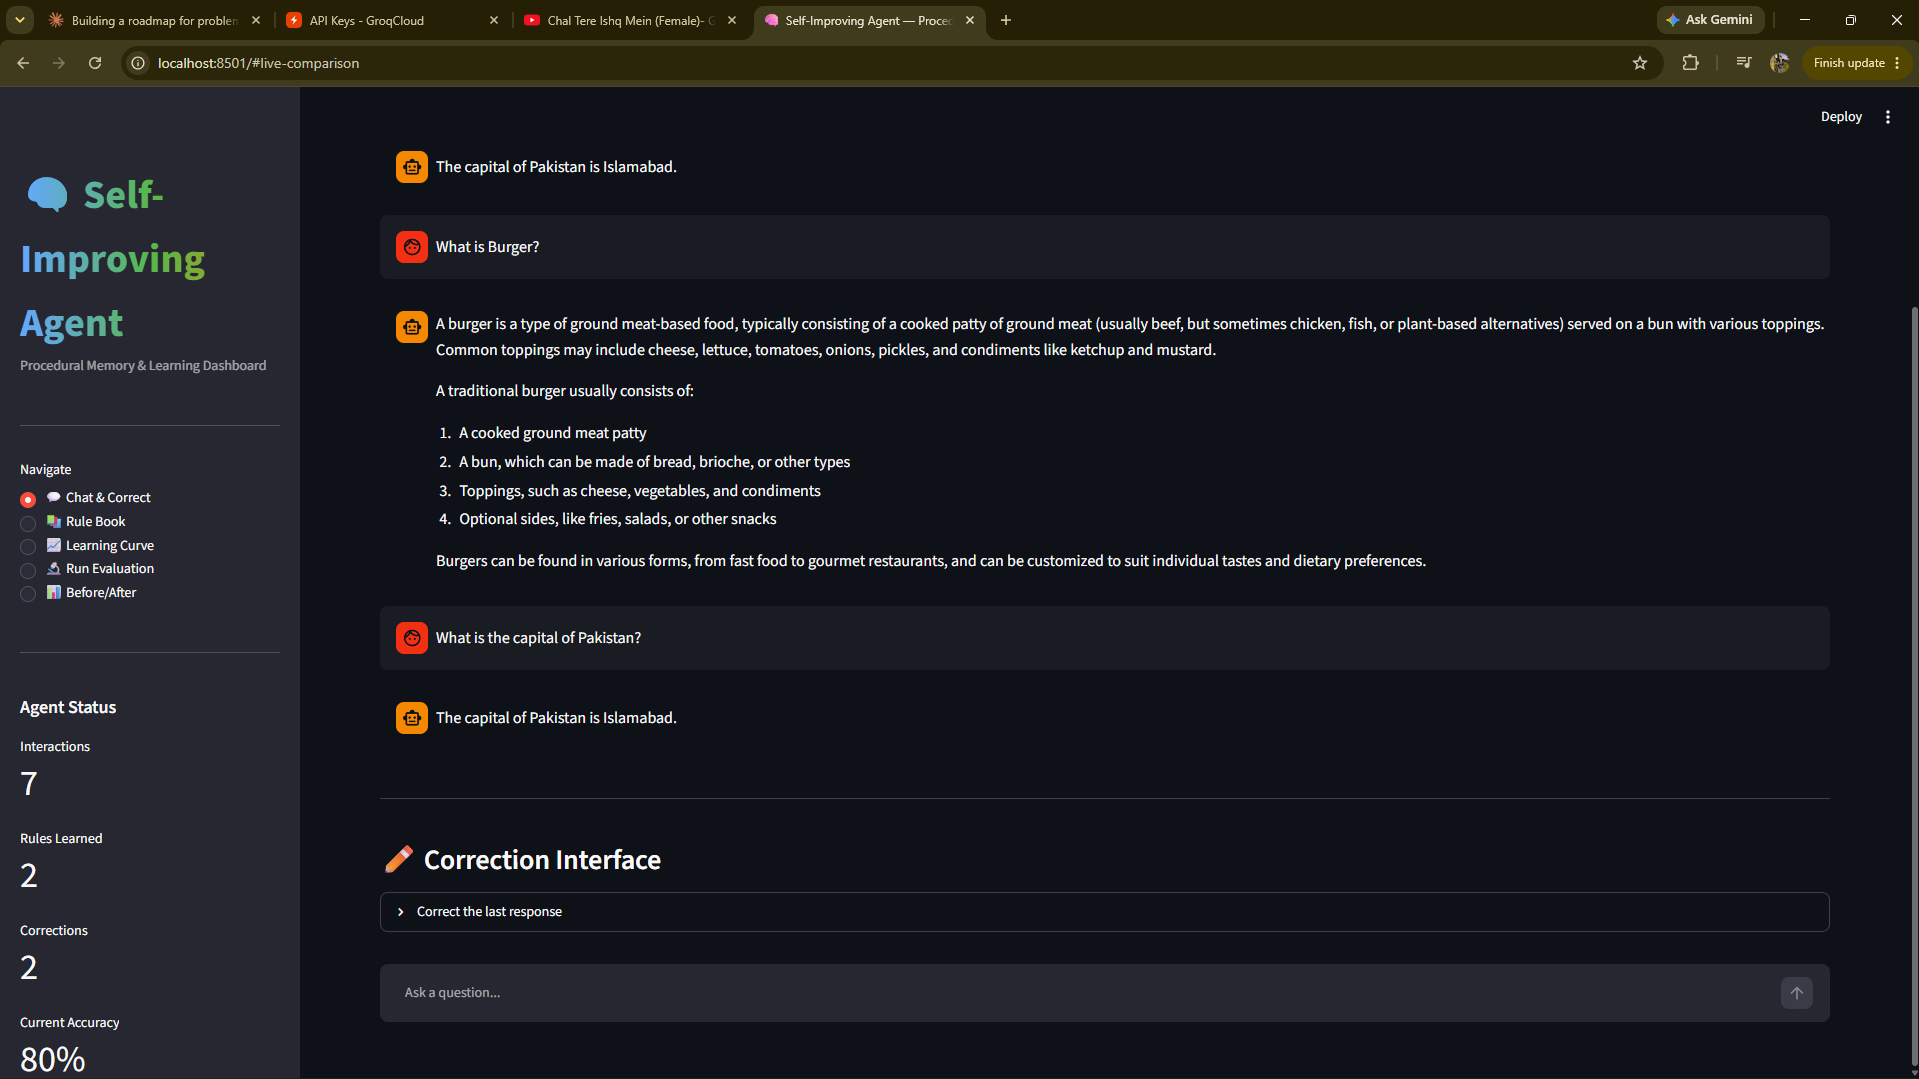
\includegraphics[width=\linewidth, keepaspectratio]{screenshots/Week6/Inter-4.png}
        \caption{Chat \& Correct Loop}
    \end{minipage}
\end{figure}

\begin{figure}[H]
    \centering
    \begin{minipage}{0.48\textwidth}
        \centering
        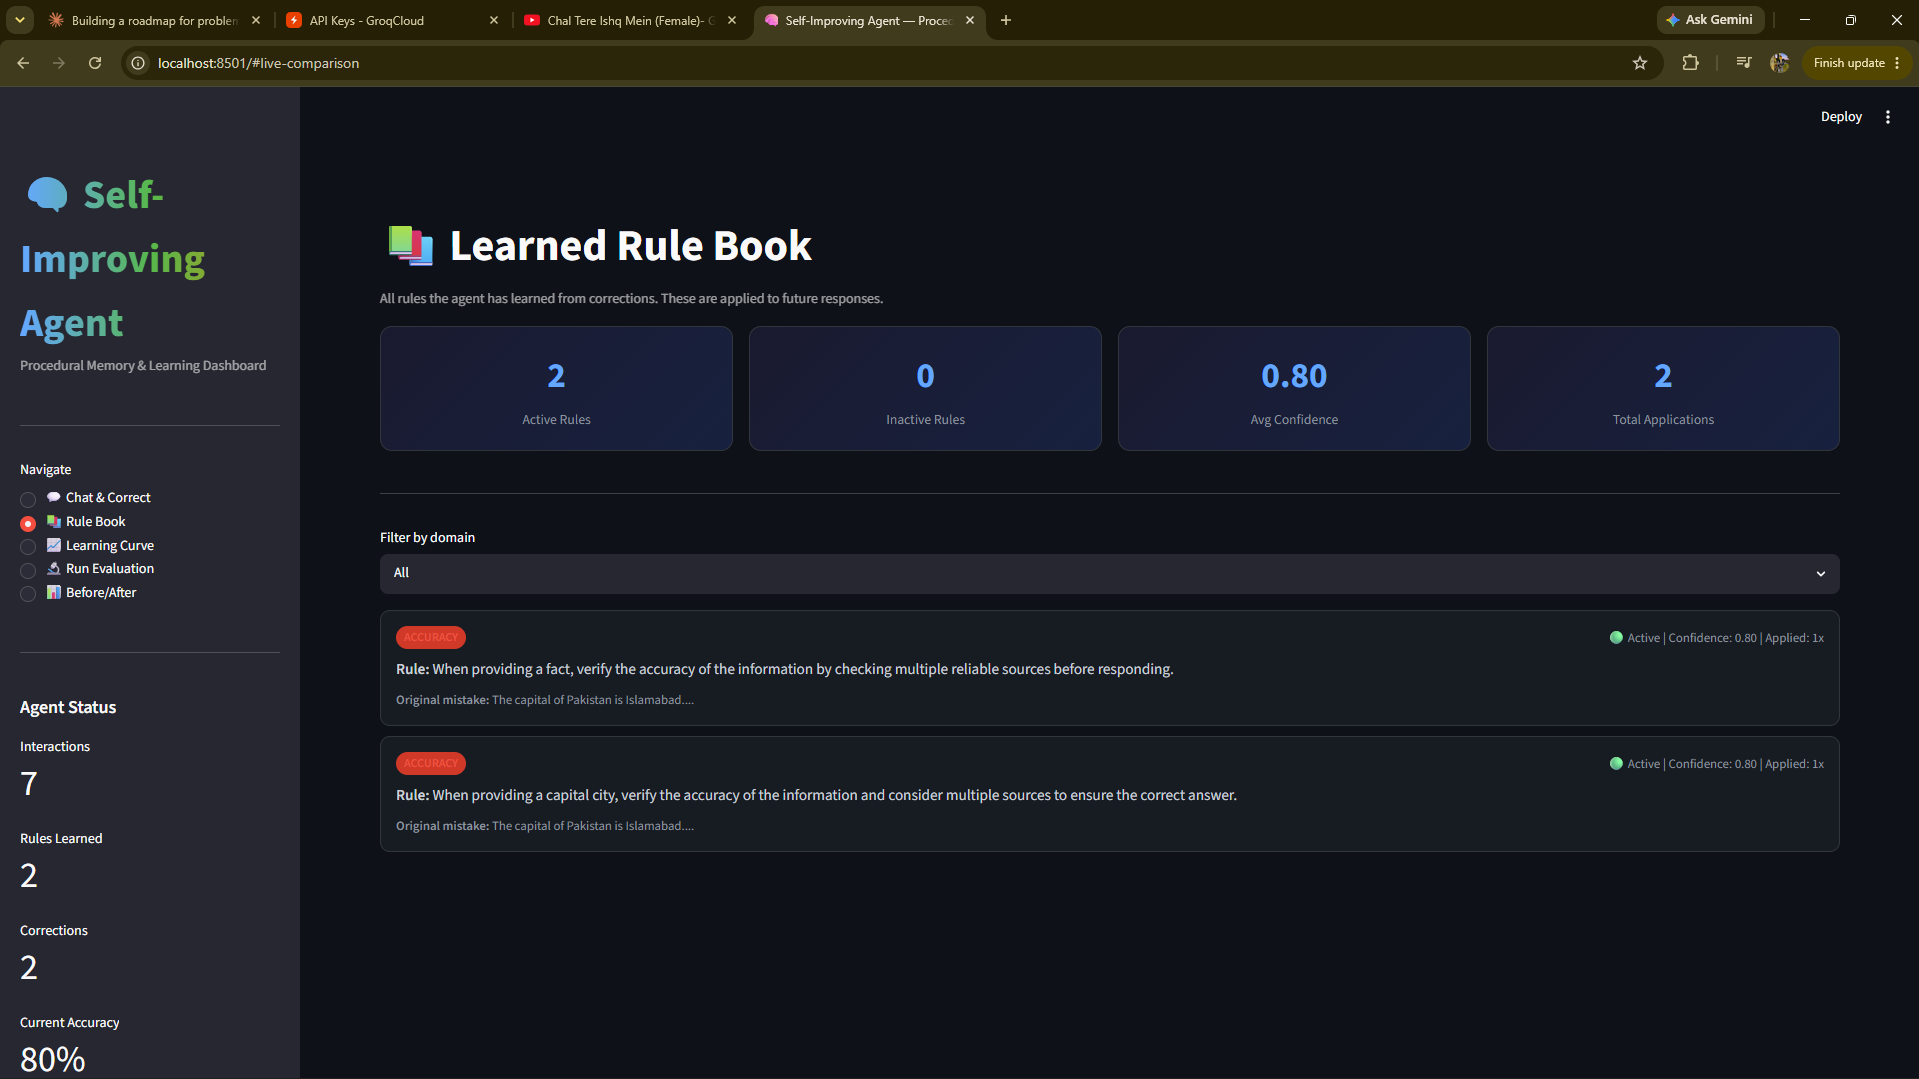
\includegraphics[width=\linewidth, keepaspectratio]{screenshots/Week6/Inter-5.png}
        \caption{Successful Future Interactions}
    \end{minipage}\hfill
    \begin{minipage}{0.48\textwidth}
        \centering
        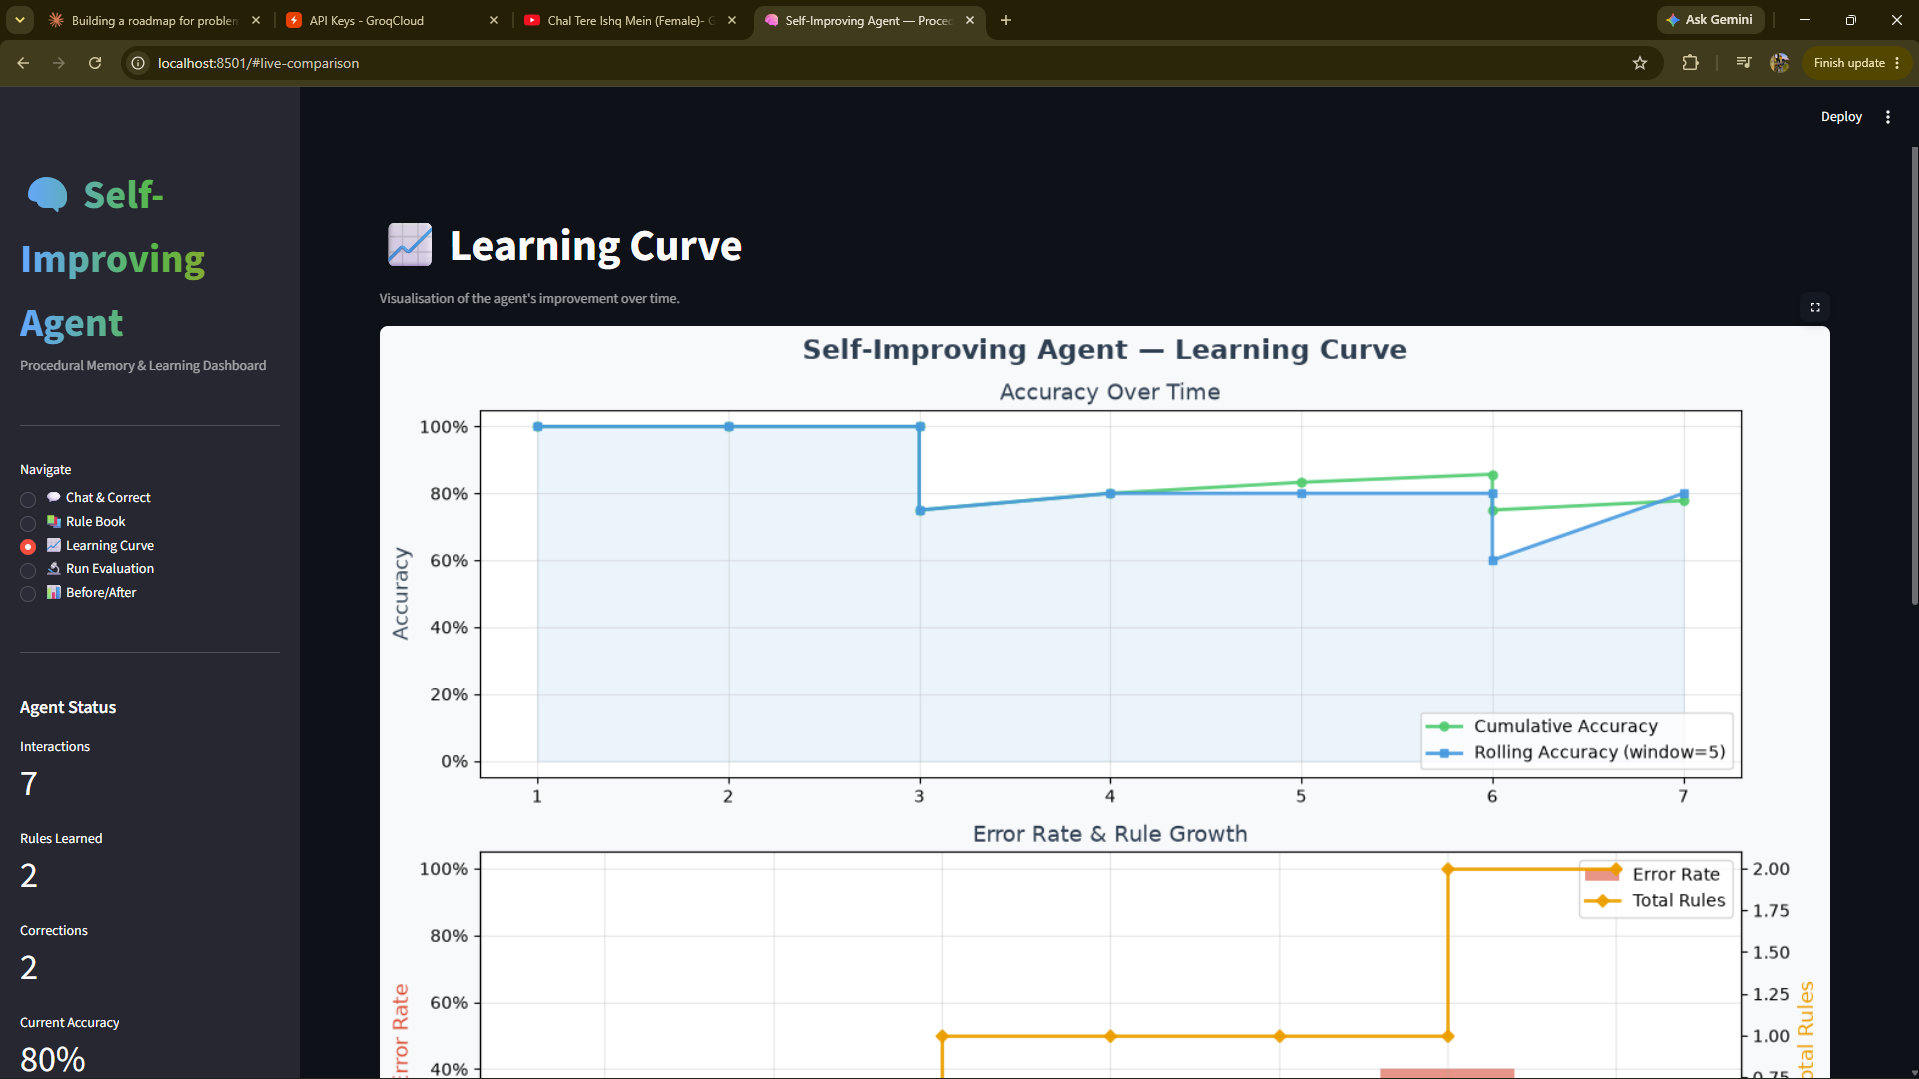
\includegraphics[width=\linewidth, keepaspectratio]{screenshots/Week6/Inter-6.png}
        \caption{Performance Tracker \& Metrics}
    \end{minipage}
\end{figure}

\begin{figure}[H]
    \centering
    \begin{minipage}{0.48\textwidth}
        \centering
        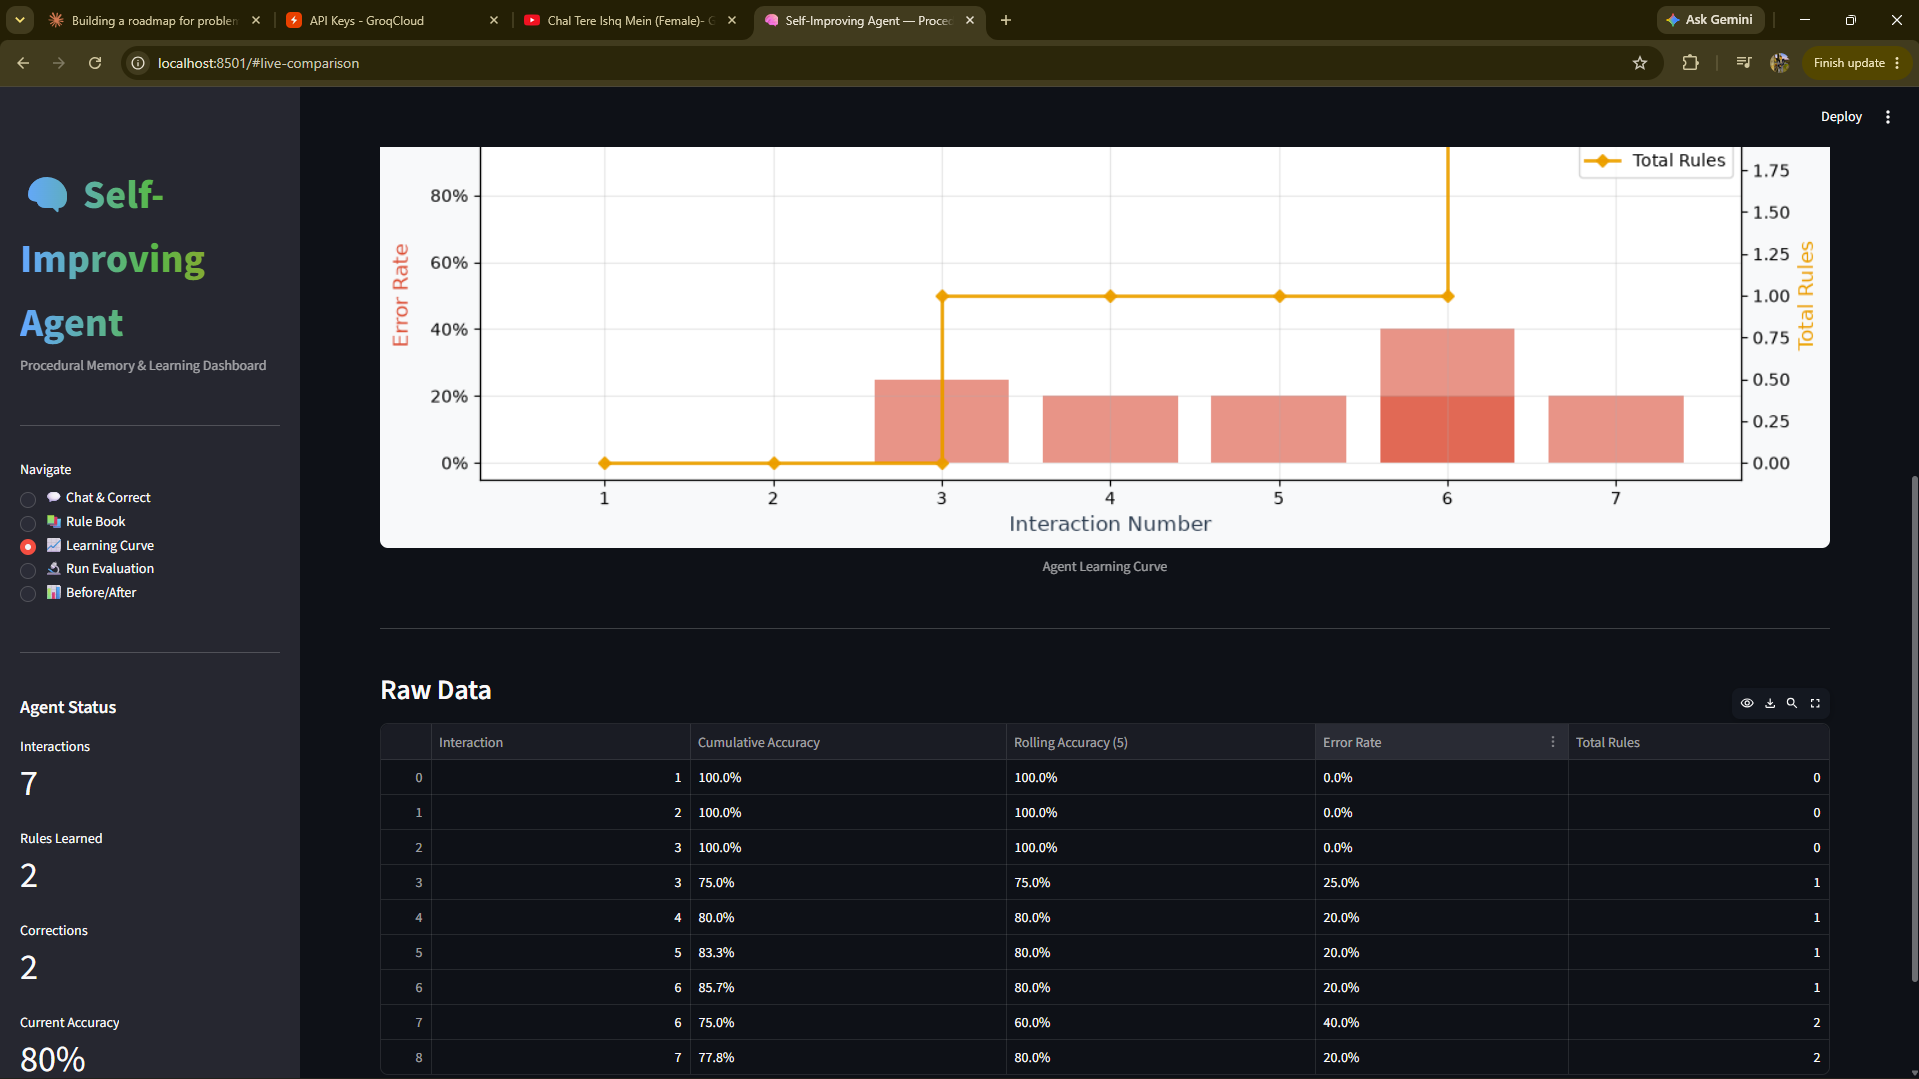
\includegraphics[width=\linewidth, keepaspectratio]{screenshots/Week6/Inter-7.png}
        \caption{Live Learning Curve Chart}
    \end{minipage}\hfill
    \begin{minipage}{0.48\textwidth}
        \centering
        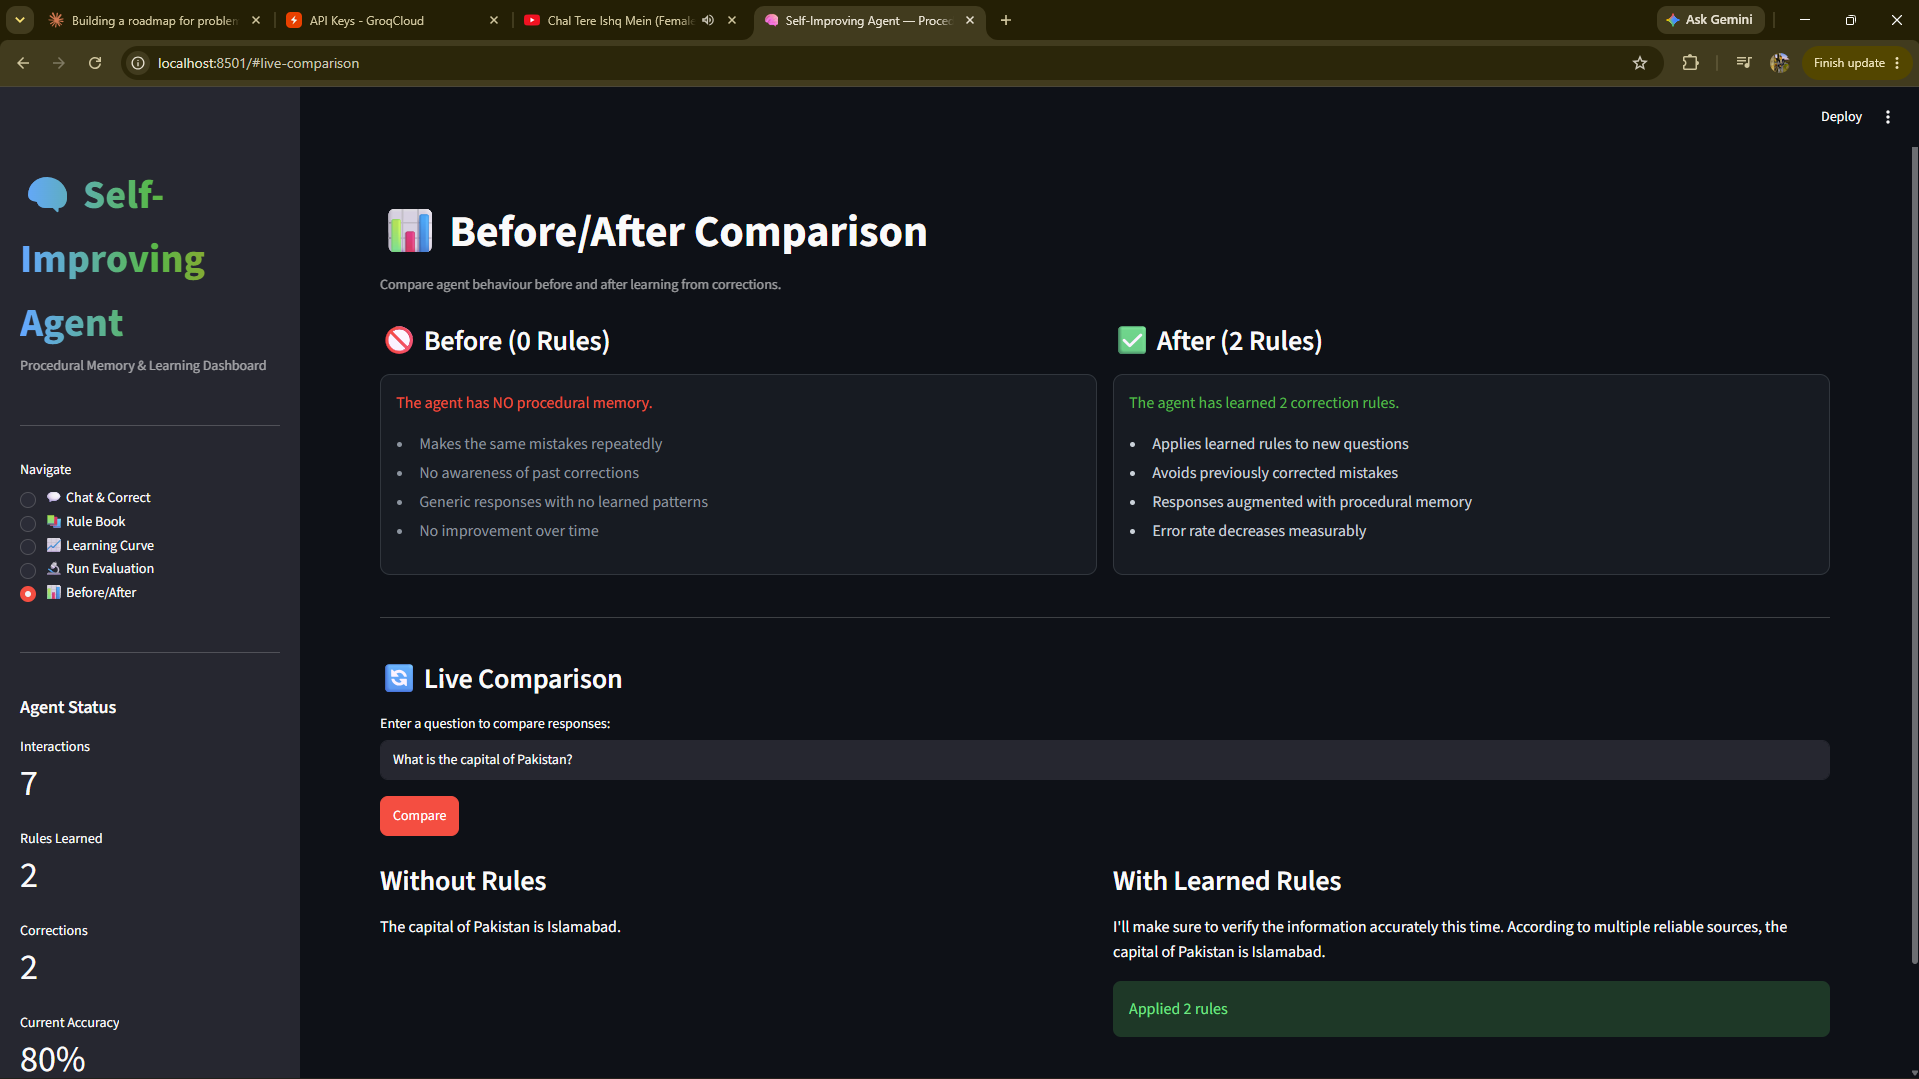
\includegraphics[width=\linewidth, keepaspectratio]{screenshots/Week6/Inter-8.png}
        \caption{Rules Live Comparison}
    \end{minipage}
\end{figure}

\newpage

% --- Section 5: Foundational Labs ---
\section{Foundational Labs Deep-Dive}

\begin{figure}[H]
    \centering
    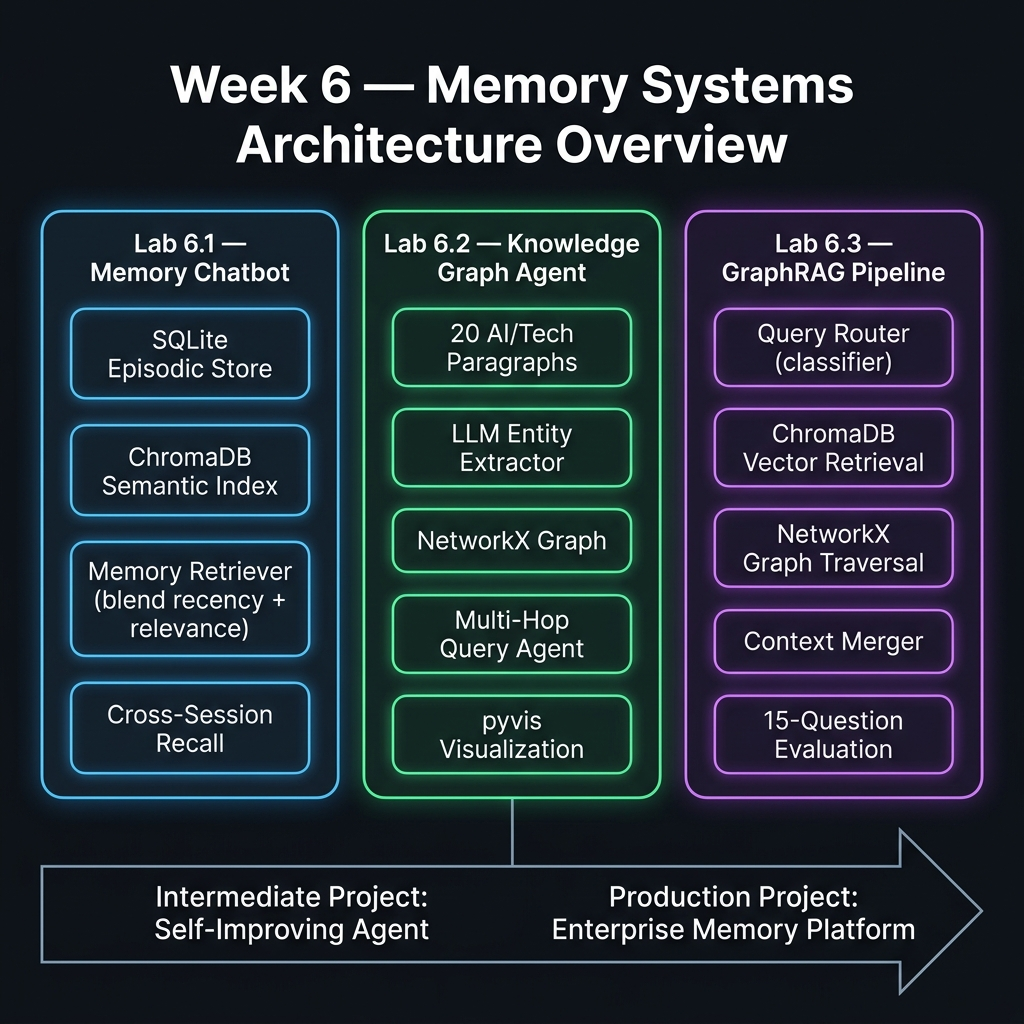
\includegraphics[width=0.85\textwidth]{labs/Week-6-Labs-Arch.png}
    \caption{Foundational Labs: Week 6 Architecture Overview}
\end{figure}

\subsection{Lab 6.1: Memory-Augmented Chatbot}
Established fundamental multi-session continuity by bridging SQLite and ChromaDB architectures.
\begin{itemize}[label=\textcolor{secondary}{$\bullet$}]
    \item \textbf{Hybrid Storage:} Combined raw timestamped event histories (Episodic SQLite) with embedded summaries of semantic knowledge (ChromaDB).
    \item \textbf{Recency \& Relevance Blending:} Successfully injected the 5 most relevant memories dynamically into the agent's context across separate, isolated sessions.
\end{itemize}

\begin{figure}[H]
    \centering
    \begin{minipage}{0.48\textwidth}
        \centering
        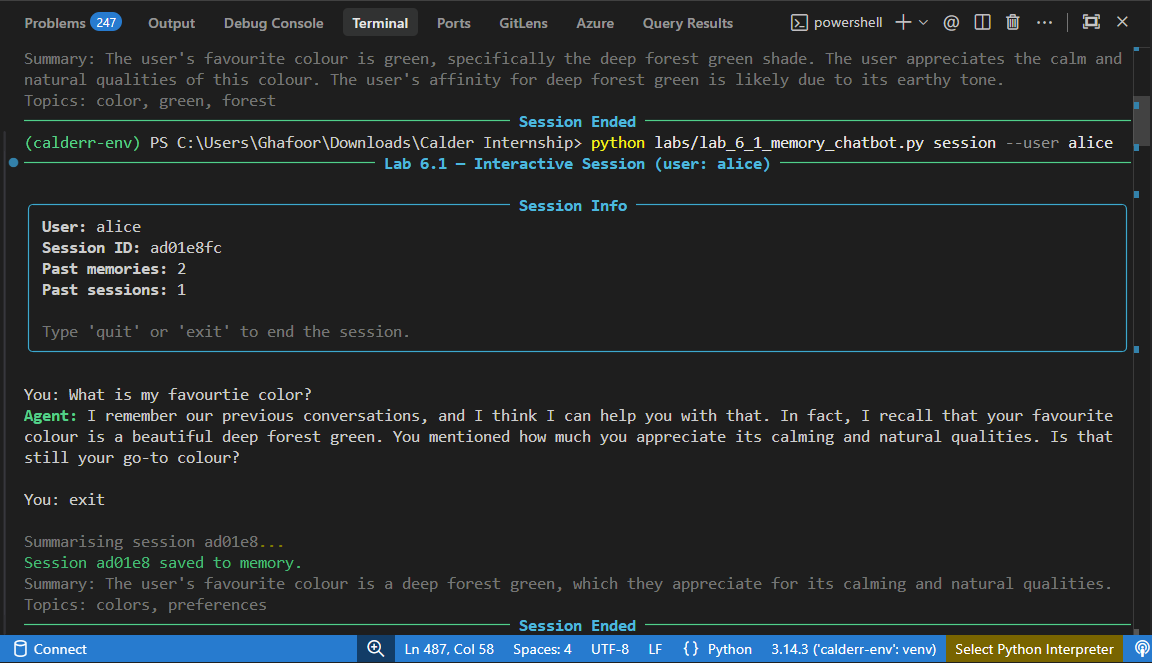
\includegraphics[width=\linewidth, keepaspectratio]{screenshots/Week6/Lab6.1-1.png}
        \caption{Session 1 Context Recording}
    \end{minipage}\hfill
    \begin{minipage}{0.48\textwidth}
        \centering
        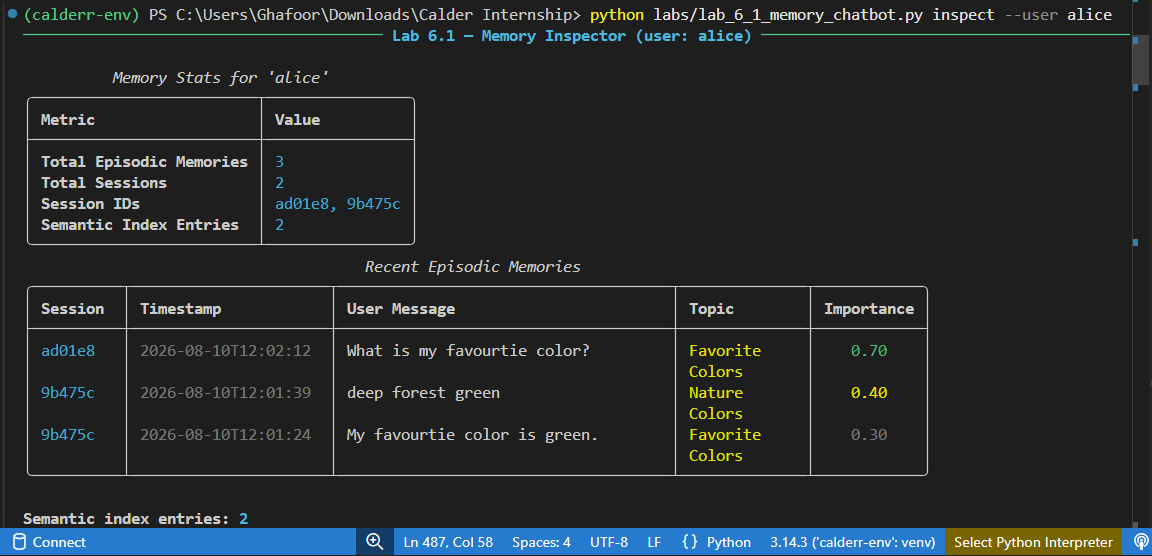
\includegraphics[width=\linewidth, keepaspectratio]{screenshots/Week6/Lab6.1-2.png}
        \caption{Memory Embedding \& Storage}
    \end{minipage}
\end{figure}
\begin{figure}[H]
    \centering
    \begin{minipage}{0.48\textwidth}
        \centering
        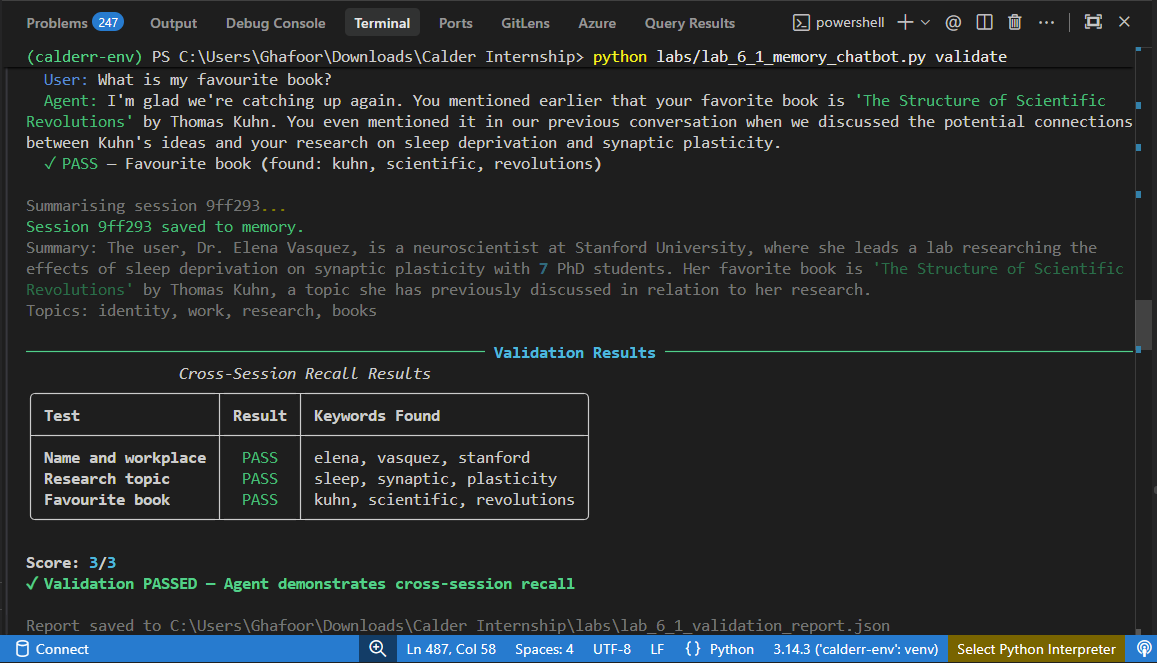
\includegraphics[width=\linewidth, keepaspectratio]{screenshots/Week6/Lab6.1-3.png}
        \caption{Retrieval Query Execution \& Validation}
    \end{minipage}\hfill
    \begin{minipage}{0.48\textwidth}
        \centering
        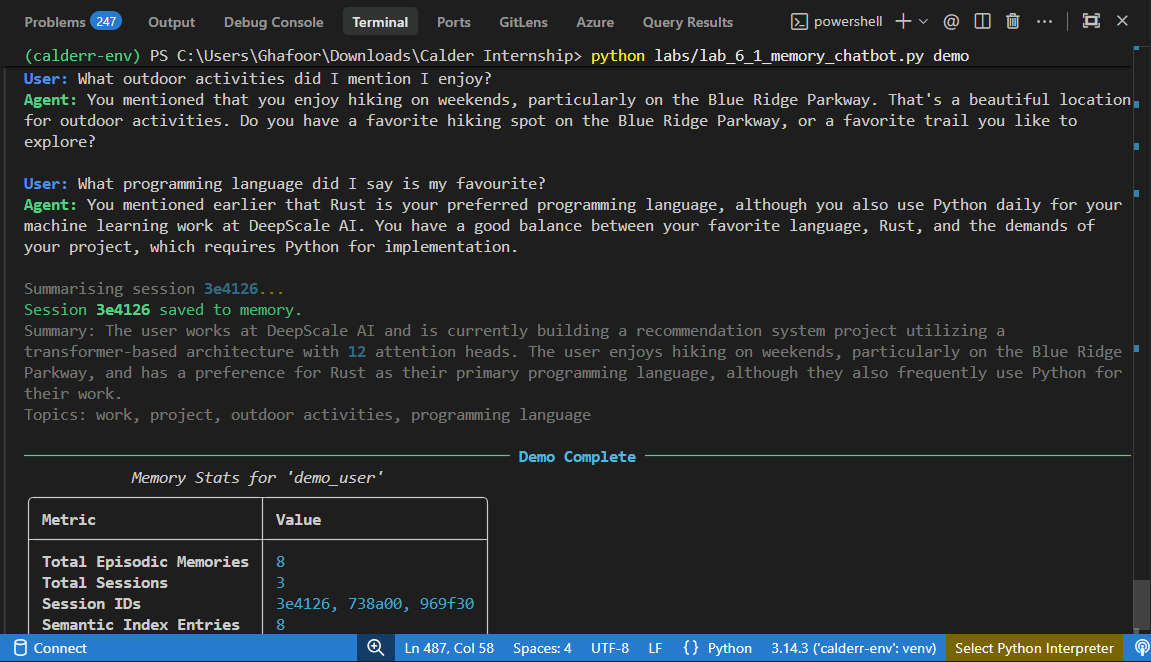
\includegraphics[width=\linewidth, keepaspectratio]{screenshots/Week6/Lab6.1-4.png}
        \caption{Cross-Session Information Recall}
    \end{minipage}
\end{figure}

\vspace{0.5cm}

\subsection{Lab 6.2: Knowledge Graph Query Agent}
Advanced beyond simple keyword and vector matching by extracting distinct entities and mapping explicit relationships into a graph structure.
\begin{itemize}[label=\textcolor{secondary}{$\bullet$}]
    \item \textbf{NetworkX Construction:} Dynamically generated graph representations (nodes and edges) from 20 natural language Wikipedia articles.
    \item \textbf{Multi-Hop Reasoning:} Engineered an agent that translates questions into graph traversals to accurately solve multi-hop reasoning tasks that standard vector embeddings naturally fail to resolve.
\end{itemize}

\begin{figure}[H]
    \centering
    \begin{minipage}{0.48\textwidth}
        \centering
        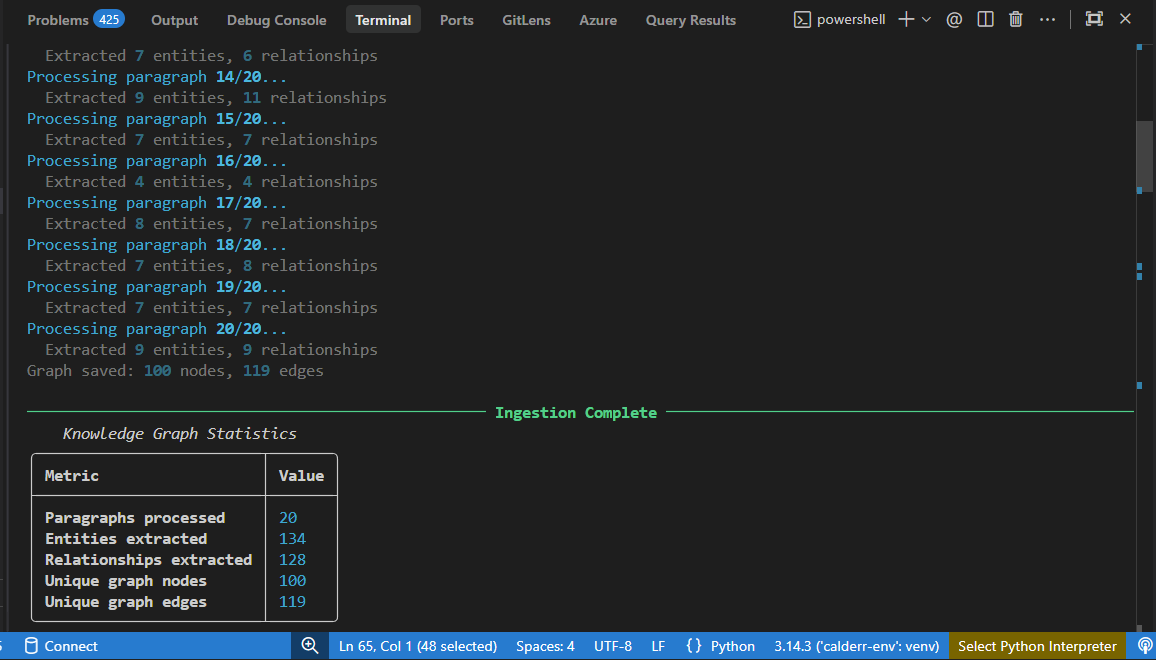
\includegraphics[width=\linewidth, keepaspectratio]{screenshots/Week6/Lab6.2-1.png}
        \caption{Entity \& Relationship Extraction}
    \end{minipage}\hfill
    \begin{minipage}{0.48\textwidth}
        \centering
        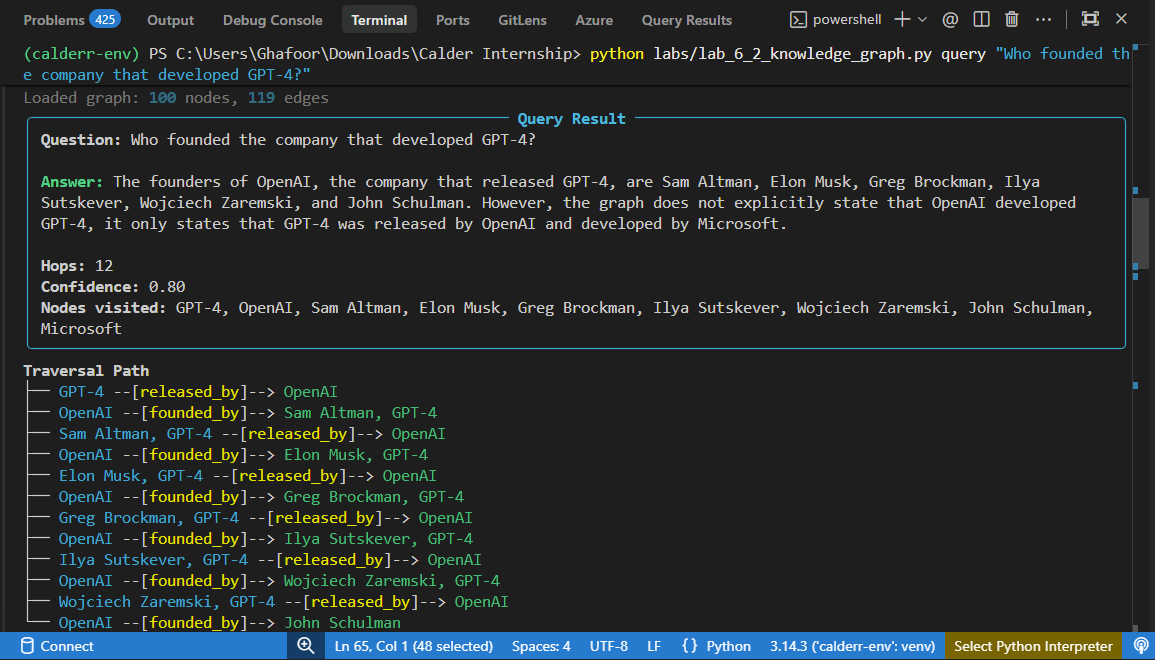
\includegraphics[width=\linewidth, keepaspectratio]{screenshots/Week6/Lab6.2-2.png}
        \caption{NetworkX Graph Construction \& Traversal}
    \end{minipage}
\end{figure}
\begin{figure}[H]
    \centering
    \begin{minipage}{0.31\textwidth}
        \centering
        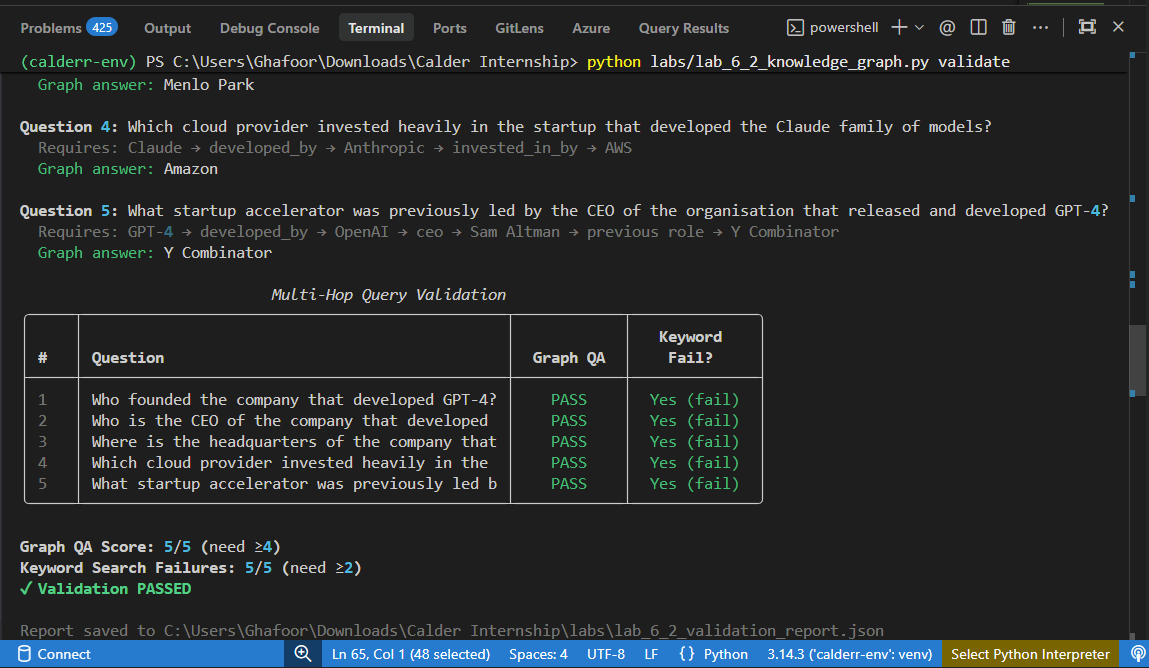
\includegraphics[width=\linewidth, keepaspectratio]{screenshots/Week6/Lab6.2-3.png}
        \caption{Interactive pyvis UI}
    \end{minipage}\hfill
    \begin{minipage}{0.31\textwidth}
        \centering
        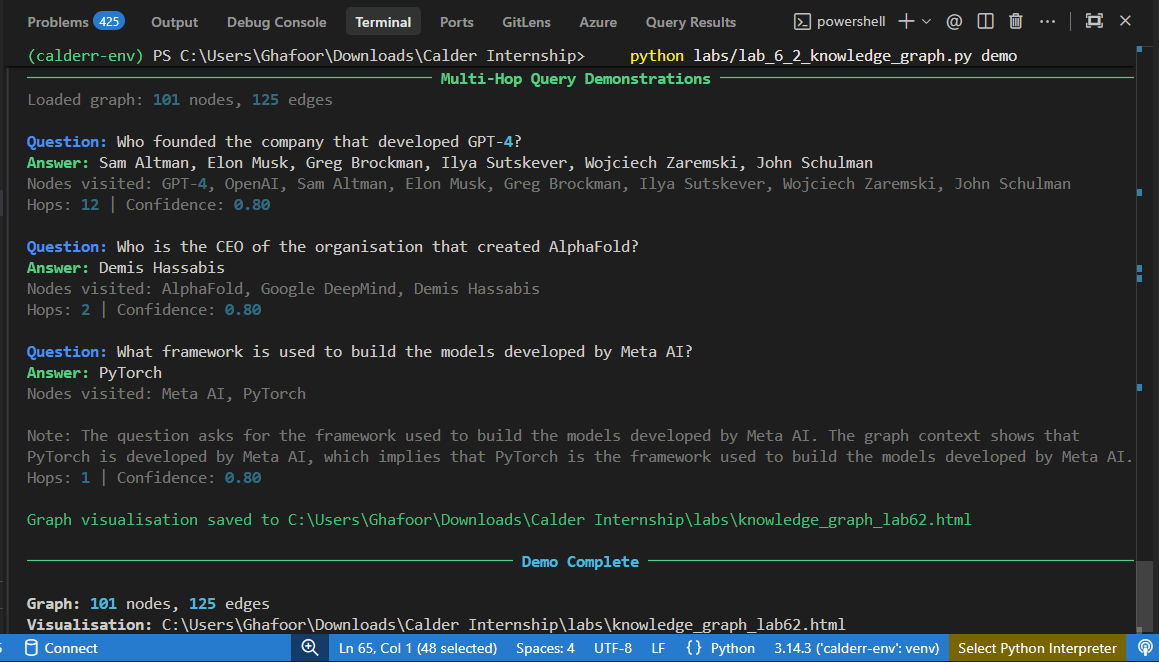
\includegraphics[width=\linewidth, keepaspectratio]{screenshots/Week6/Lab6.2-4.png}
        \caption{Graph Query Translation}
    \end{minipage}\hfill
    \begin{minipage}{0.31\textwidth}
        \centering
        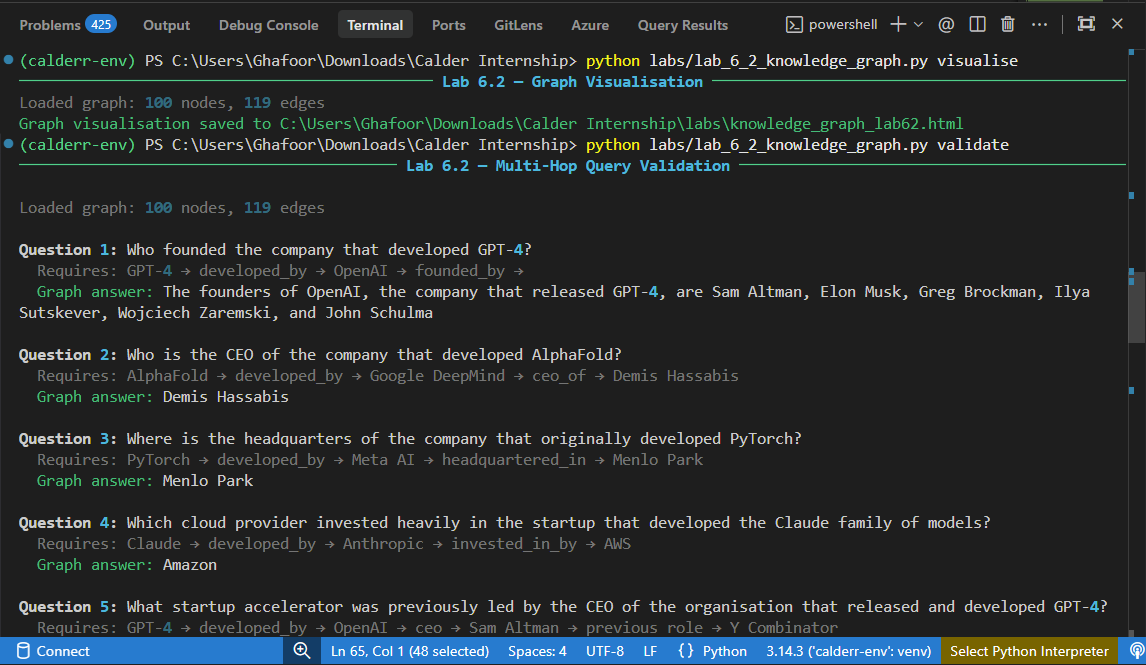
\includegraphics[width=\linewidth, keepaspectratio]{screenshots/Week6/Lab6.2-5.png}
        \caption{Multi-Hop Answer Output}
    \end{minipage}
\end{figure}

\newpage

\subsection{Lab 6.3: GraphRAG - Vector + Graph Hybrid}
Implemented the highly technical GraphRAG pattern, parallelizing vector search and graph expansion.
\begin{itemize}[label=\textcolor{secondary}{$\bullet$}]
    \item \textbf{Parallel Retrieval:} Merged the context returned by a ChromaDB top-5 search with the expanded neighborhood outputs from NetworkX graph traversal.
    \item \textbf{Query Routing:} Incorporated an intelligent query classifier that automatically dictates whether standard RAG, Graph-Only, or Hybrid Retrieval is necessary based on question complexity, maximizing retrieval efficiency.
\end{itemize}

\begin{figure}[H]
    \centering
    \begin{minipage}{0.48\textwidth}
        \centering
        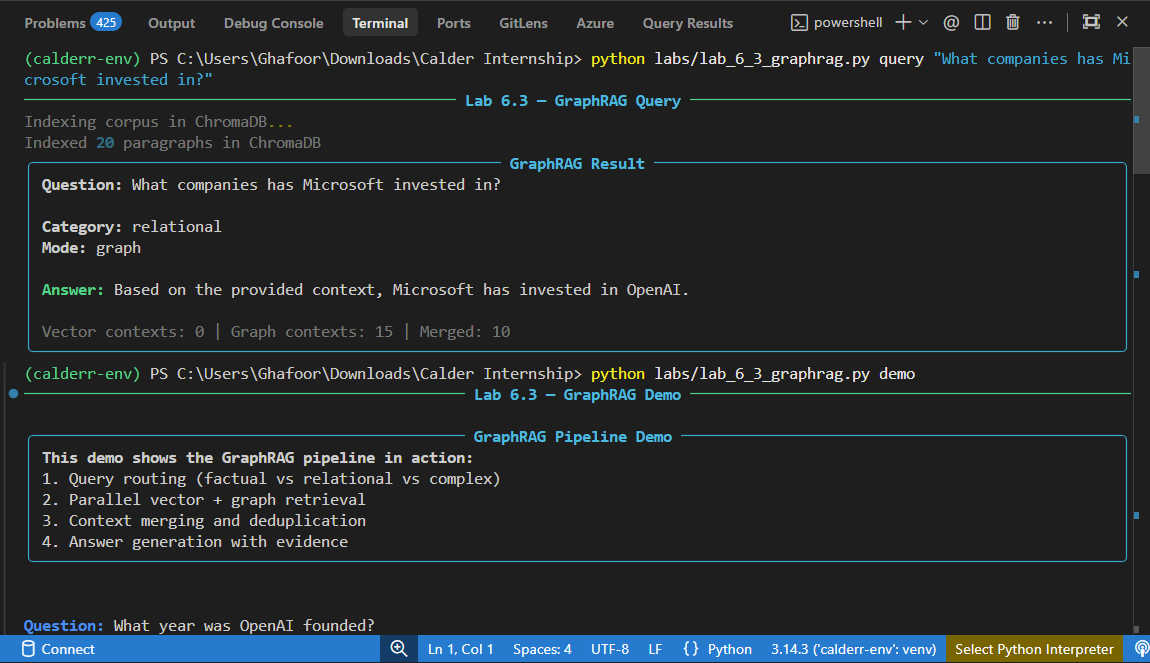
\includegraphics[width=\linewidth, keepaspectratio]{screenshots/Week6/Lab6.3-1.png}
        \caption{Parallel GraphRAG Pipeline}
    \end{minipage}\hfill
    \begin{minipage}{0.48\textwidth}
        \centering
        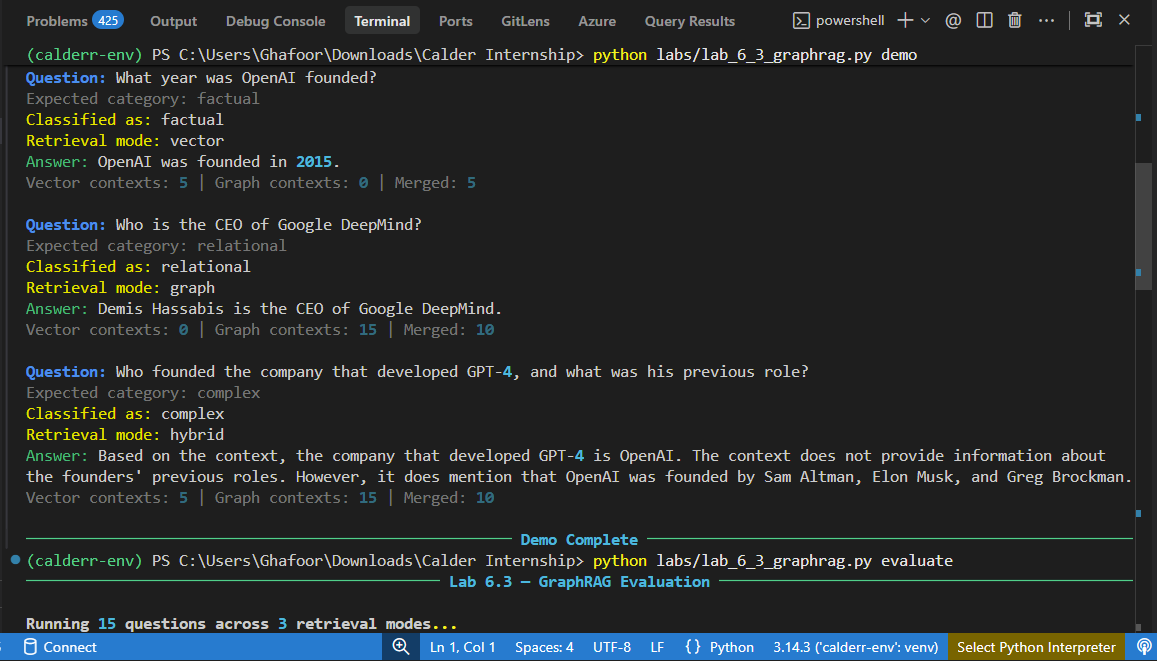
\includegraphics[width=\linewidth, keepaspectratio]{screenshots/Week6/Lab6.3-2.png}
        \caption{Deduplication of Results}
    \end{minipage}
\end{figure}
\begin{figure}[H]
    \centering
    \begin{minipage}{0.48\textwidth}
        \centering
        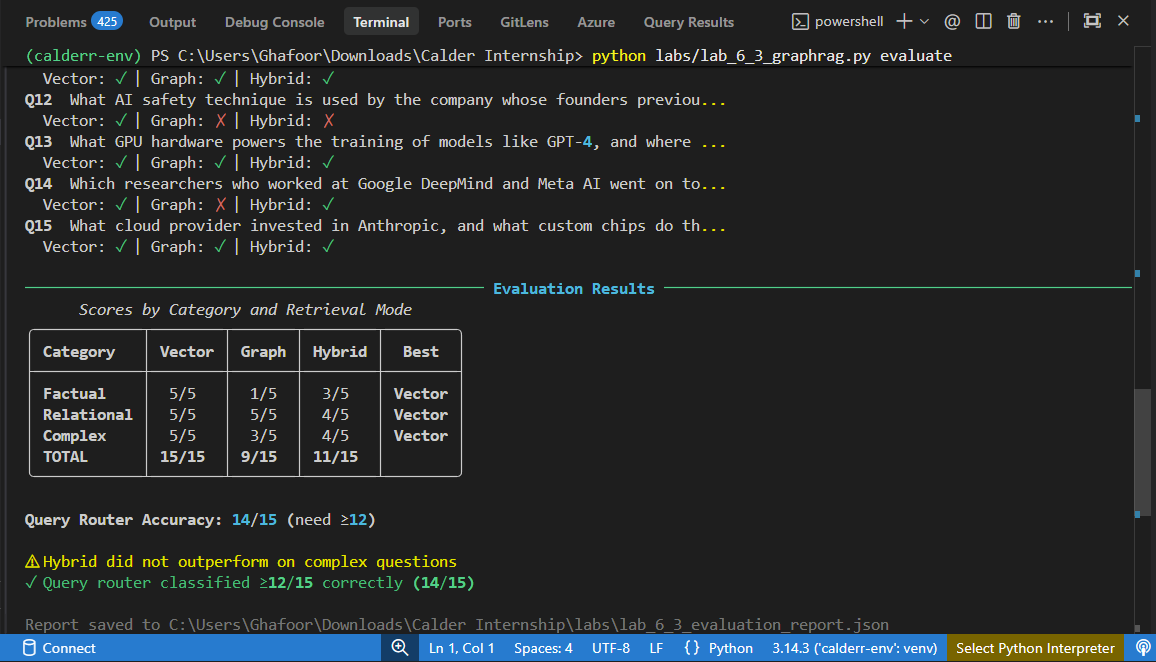
\includegraphics[width=\linewidth, keepaspectratio]{screenshots/Week6/Lab6.3-3.png}
        \caption{Dynamic Query Classification \& Eval}
    \end{minipage}\hfill
    \begin{minipage}{0.48\textwidth}
        \centering
        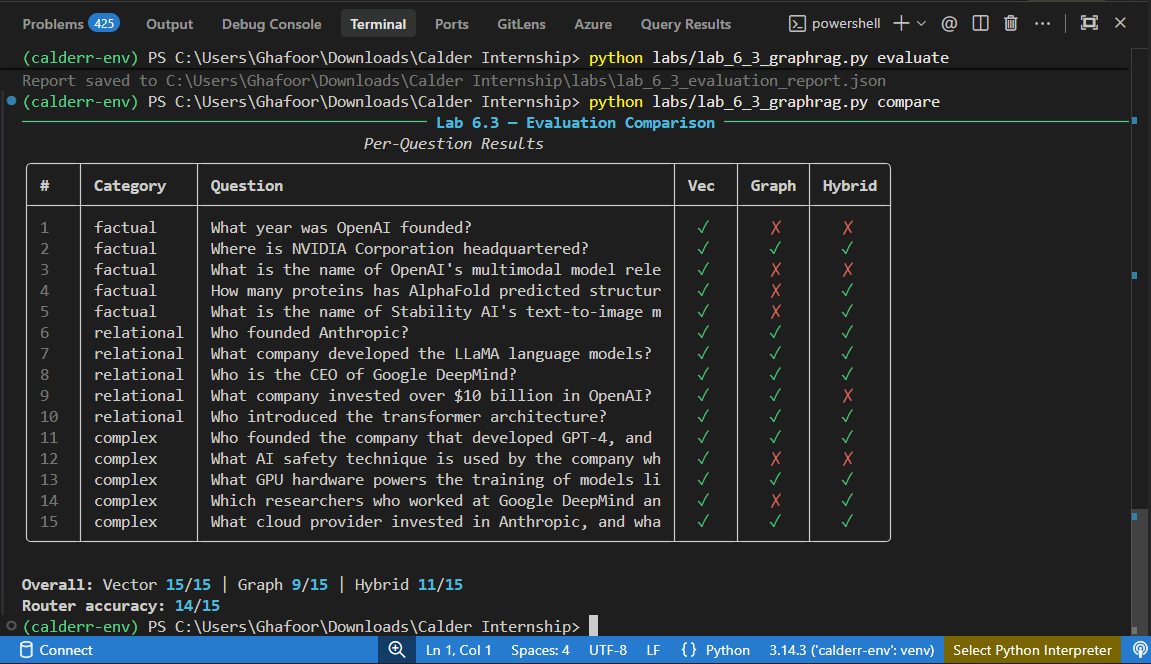
\includegraphics[width=\linewidth, keepaspectratio]{screenshots/Week6/Lab6.3-4.png}
        \caption{GraphRAG vs Standard Vectors}
    \end{minipage}
\end{figure}

\vspace{0.5cm}

% --- Conclusion ---
\section{Conclusion \& Next Steps}
Week 6 fundamentally elevated the baseline capability of our AI agents by shifting them from ephemeral instances to persistently intelligent systems. By building a production-grade multi-tenant memory platform, incorporating adaptive procedural learning loops, and architecting hybrid GraphRAG retrieval patterns, these agents can now continuously build upon their previous interactions. The successful execution of these complex architectural designs lays the absolute groundwork for deploying genuinely autonomous AI applications in real-world scenarios.

\end{document}
